\chapter{Muon background from the Beam Delivery System}
\label{Appendix:BDS_Muons}
Figure~\ref{fig:BDS_Muons:occupancies} shows occupancy plots belonging to the study presented in Chapter~\ref{BDS_Muons}.
  \begin{figure}[htbp]
 \centering
  \begin{subfigure}[b]{0.49\textwidth}
   \centering
    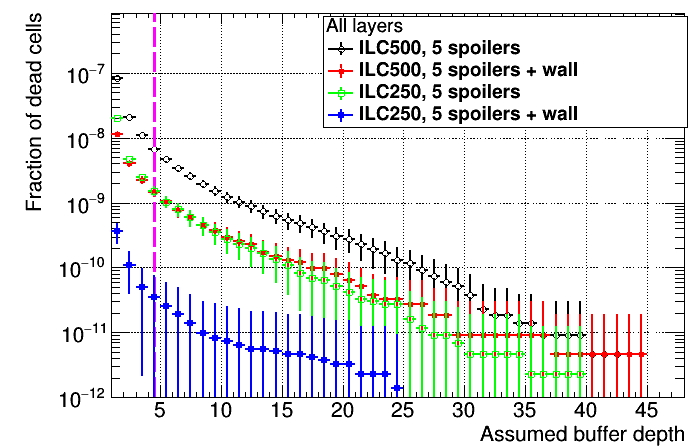
\includegraphics[width=\textwidth]{Figures/BDS_muons/Occupancy_Comparison_All_layers_deadcells_SiTrackerBarrel.png}
   \caption{Tracker barrel}
   \end{subfigure}
   \hfill
    \begin{subfigure}[b]{0.49\textwidth}
   \centering
    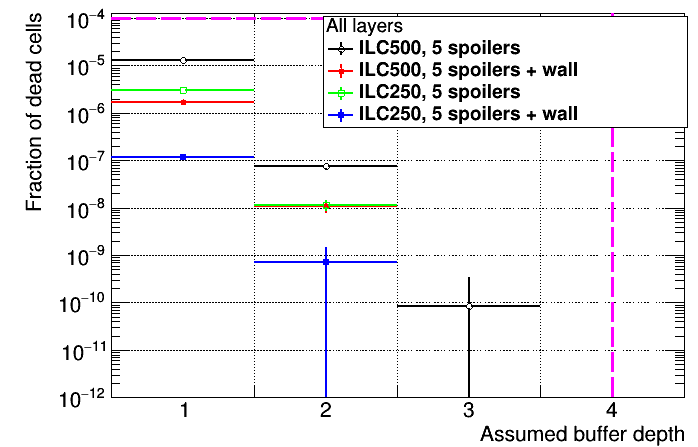
\includegraphics[width=\textwidth]{Figures/BDS_muons/Occupancy_Comparison_All_layers_deadcells_EcalBarrel.png}
   \caption{ECAL barrel}
   \end{subfigure}
  \end{figure}
  \begin{figure}[htb]\ContinuedFloat
   \begin{subfigure}[b]{0.49\textwidth}
   \centering
    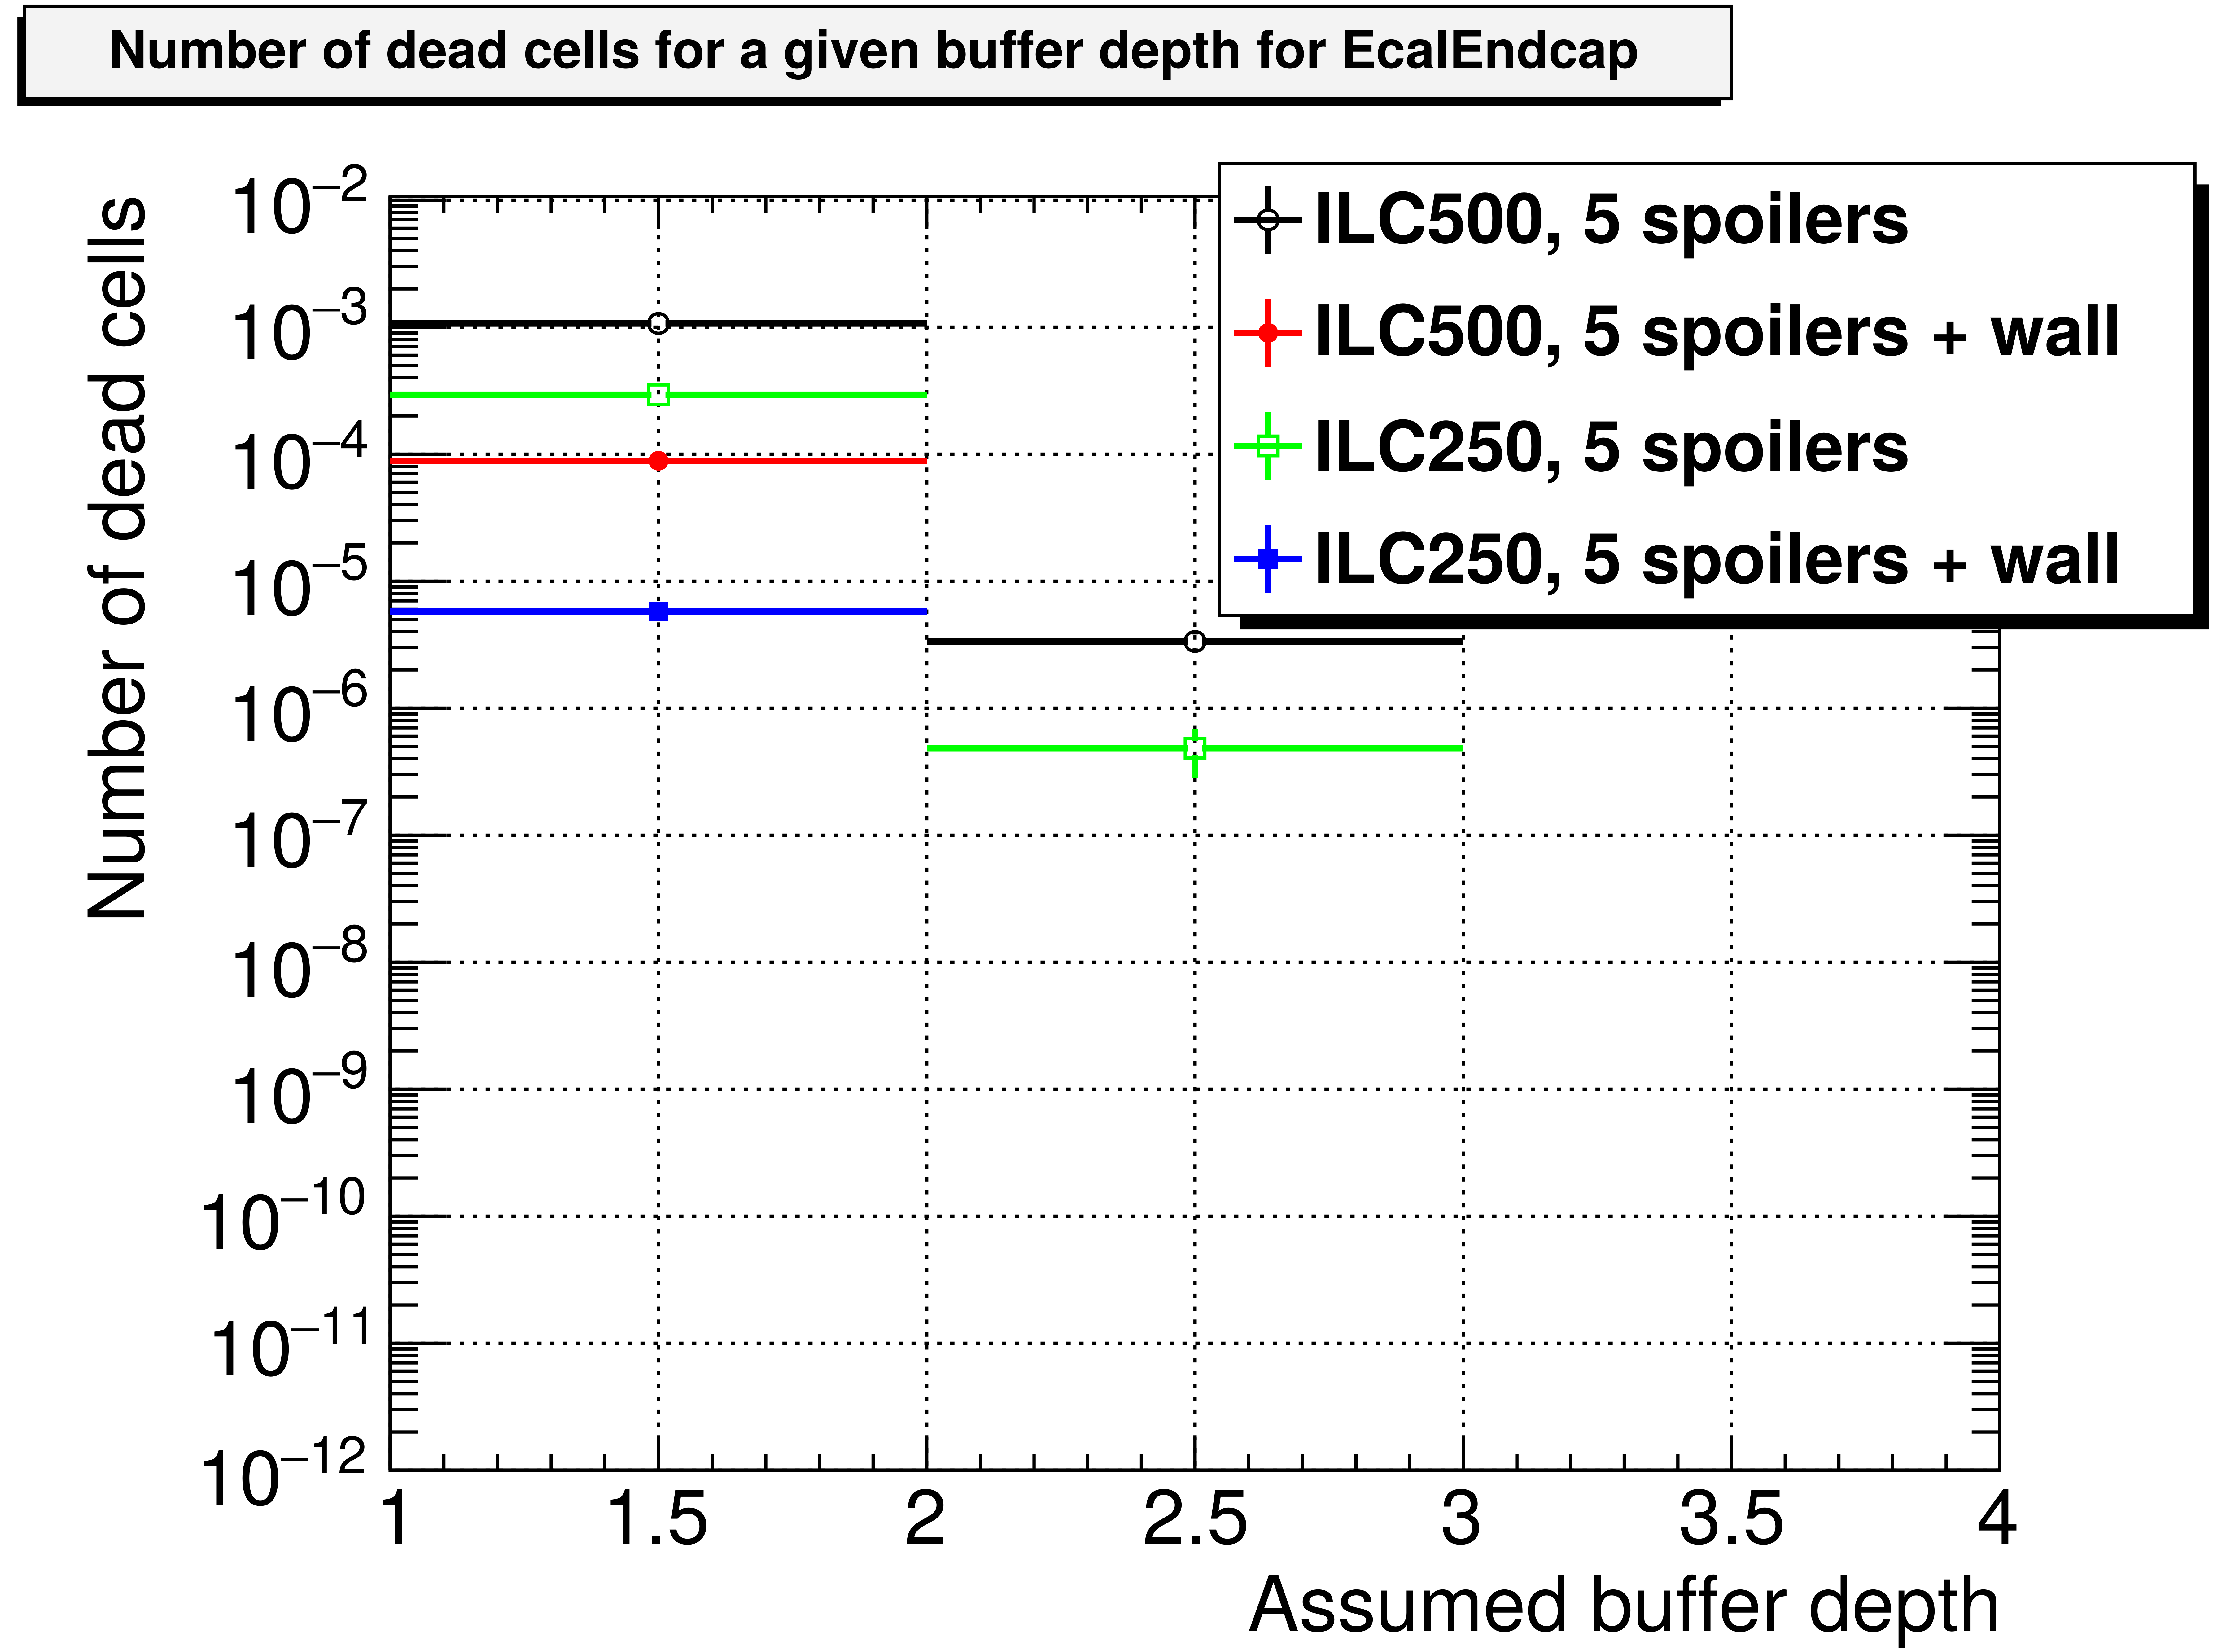
\includegraphics[width=\textwidth]{Figures/BDS_muons/Occupancy_Comparison_All_layers_deadcells_EcalEndcap.png}
   \caption{ECAL endcap}
   \end{subfigure}
   \hfill
    \begin{subfigure}[b]{0.49\textwidth}
   \centering
    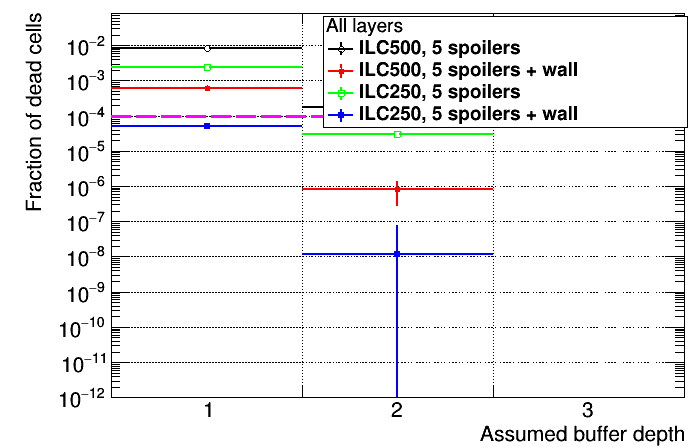
\includegraphics[width=\textwidth]{Figures/BDS_muons/Occupancy_Comparison_All_layers_deadcells_HcalEndcap.png}
   \caption{HCAL endcap}
   \end{subfigure}\\
   \begin{subfigure}[b]{0.49\textwidth}
   \centering
    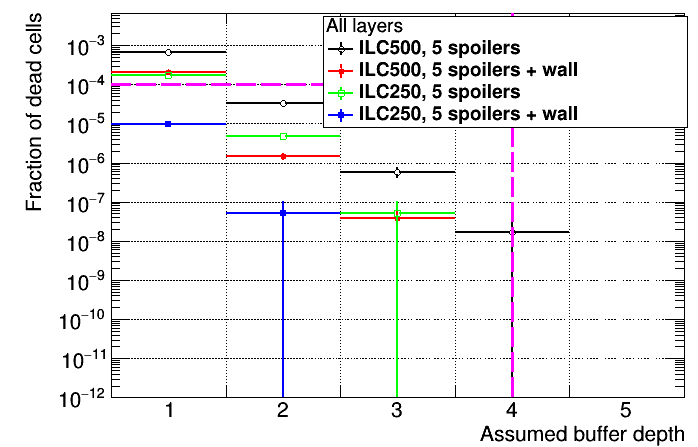
\includegraphics[width=\textwidth]{Figures/BDS_muons/Occupancy_Comparison_All_layers_deadcells_MuonBarrel.png}
   \caption{Muon system barrel}
   \end{subfigure}
   \hfill
    \begin{subfigure}[b]{0.49\textwidth}
   \centering
    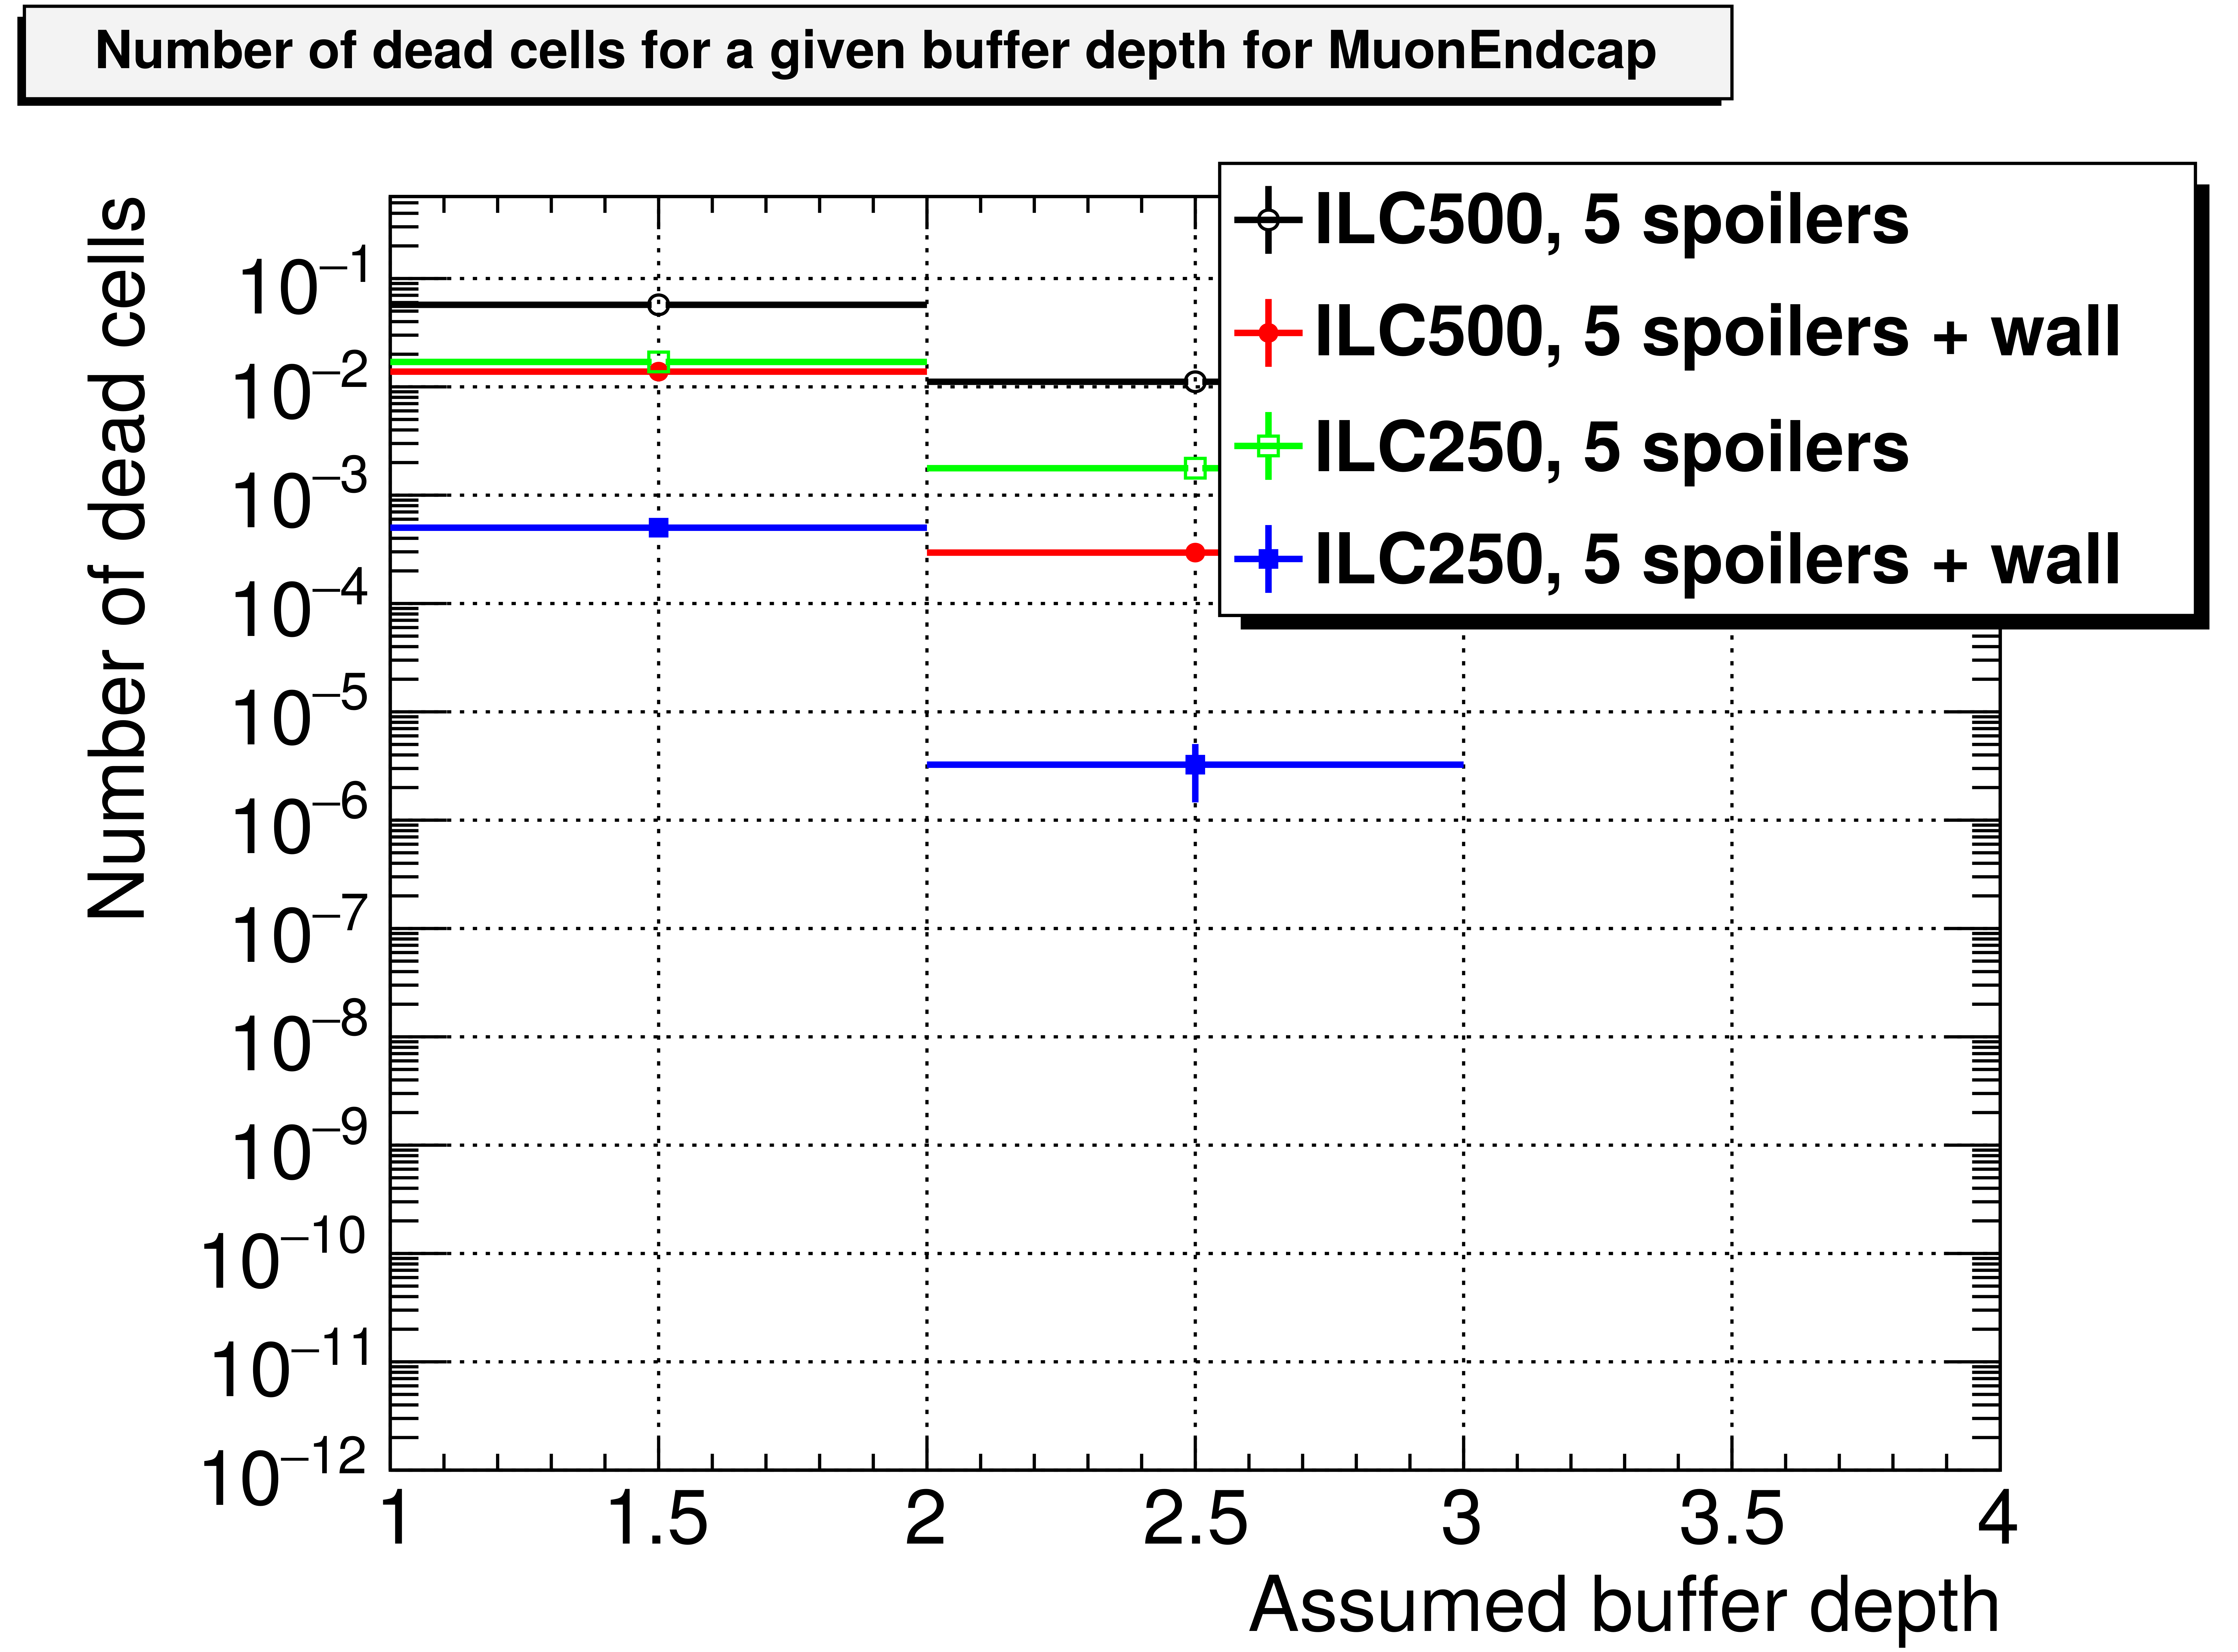
\includegraphics[width=\textwidth]{Figures/BDS_muons/Occupancy_Comparison_All_layers_deadcells_MuonEndcap.png}
   \caption{Muon system endcap}
   \end{subfigure}\\
     \begin{subfigure}[b]{0.49\textwidth}
   \centering
    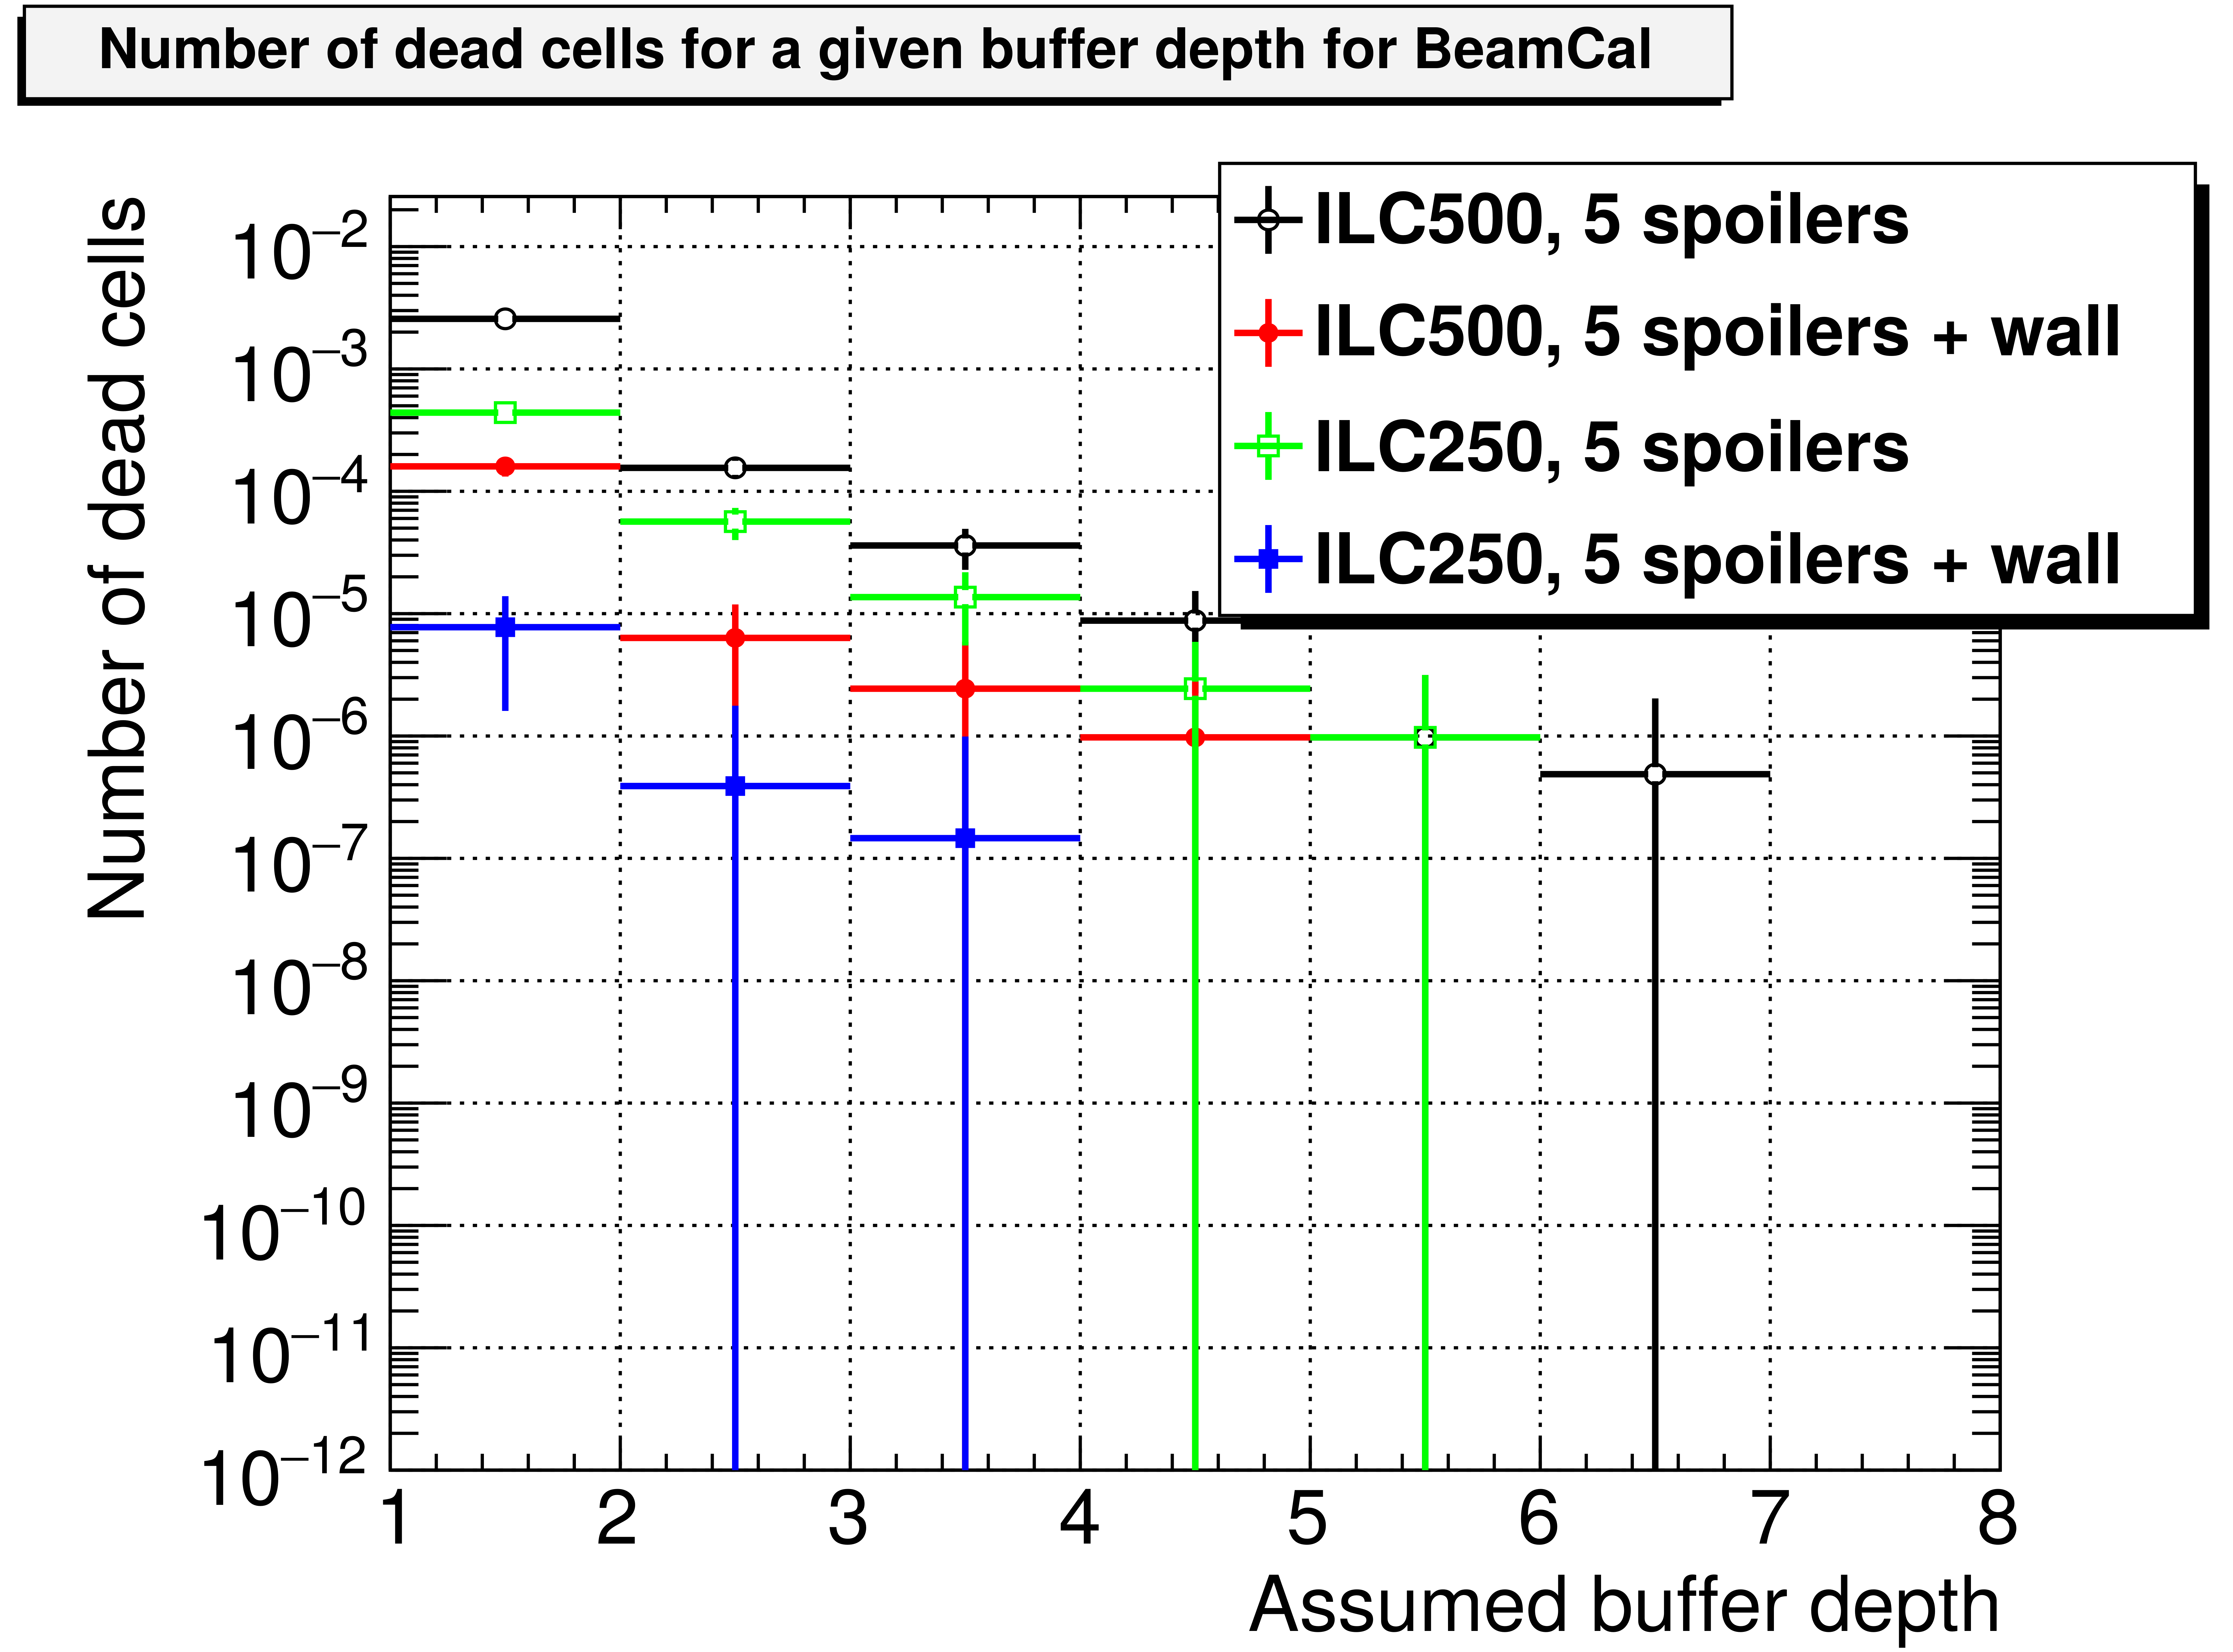
\includegraphics[width=\textwidth]{Figures/BDS_muons/Occupancy_Comparison_All_layers_deadcells_BeamCal.png}
   \caption{BeamCal}
   \end{subfigure}
   \hfill
    \begin{subfigure}[b]{0.49\textwidth}
   \centering
    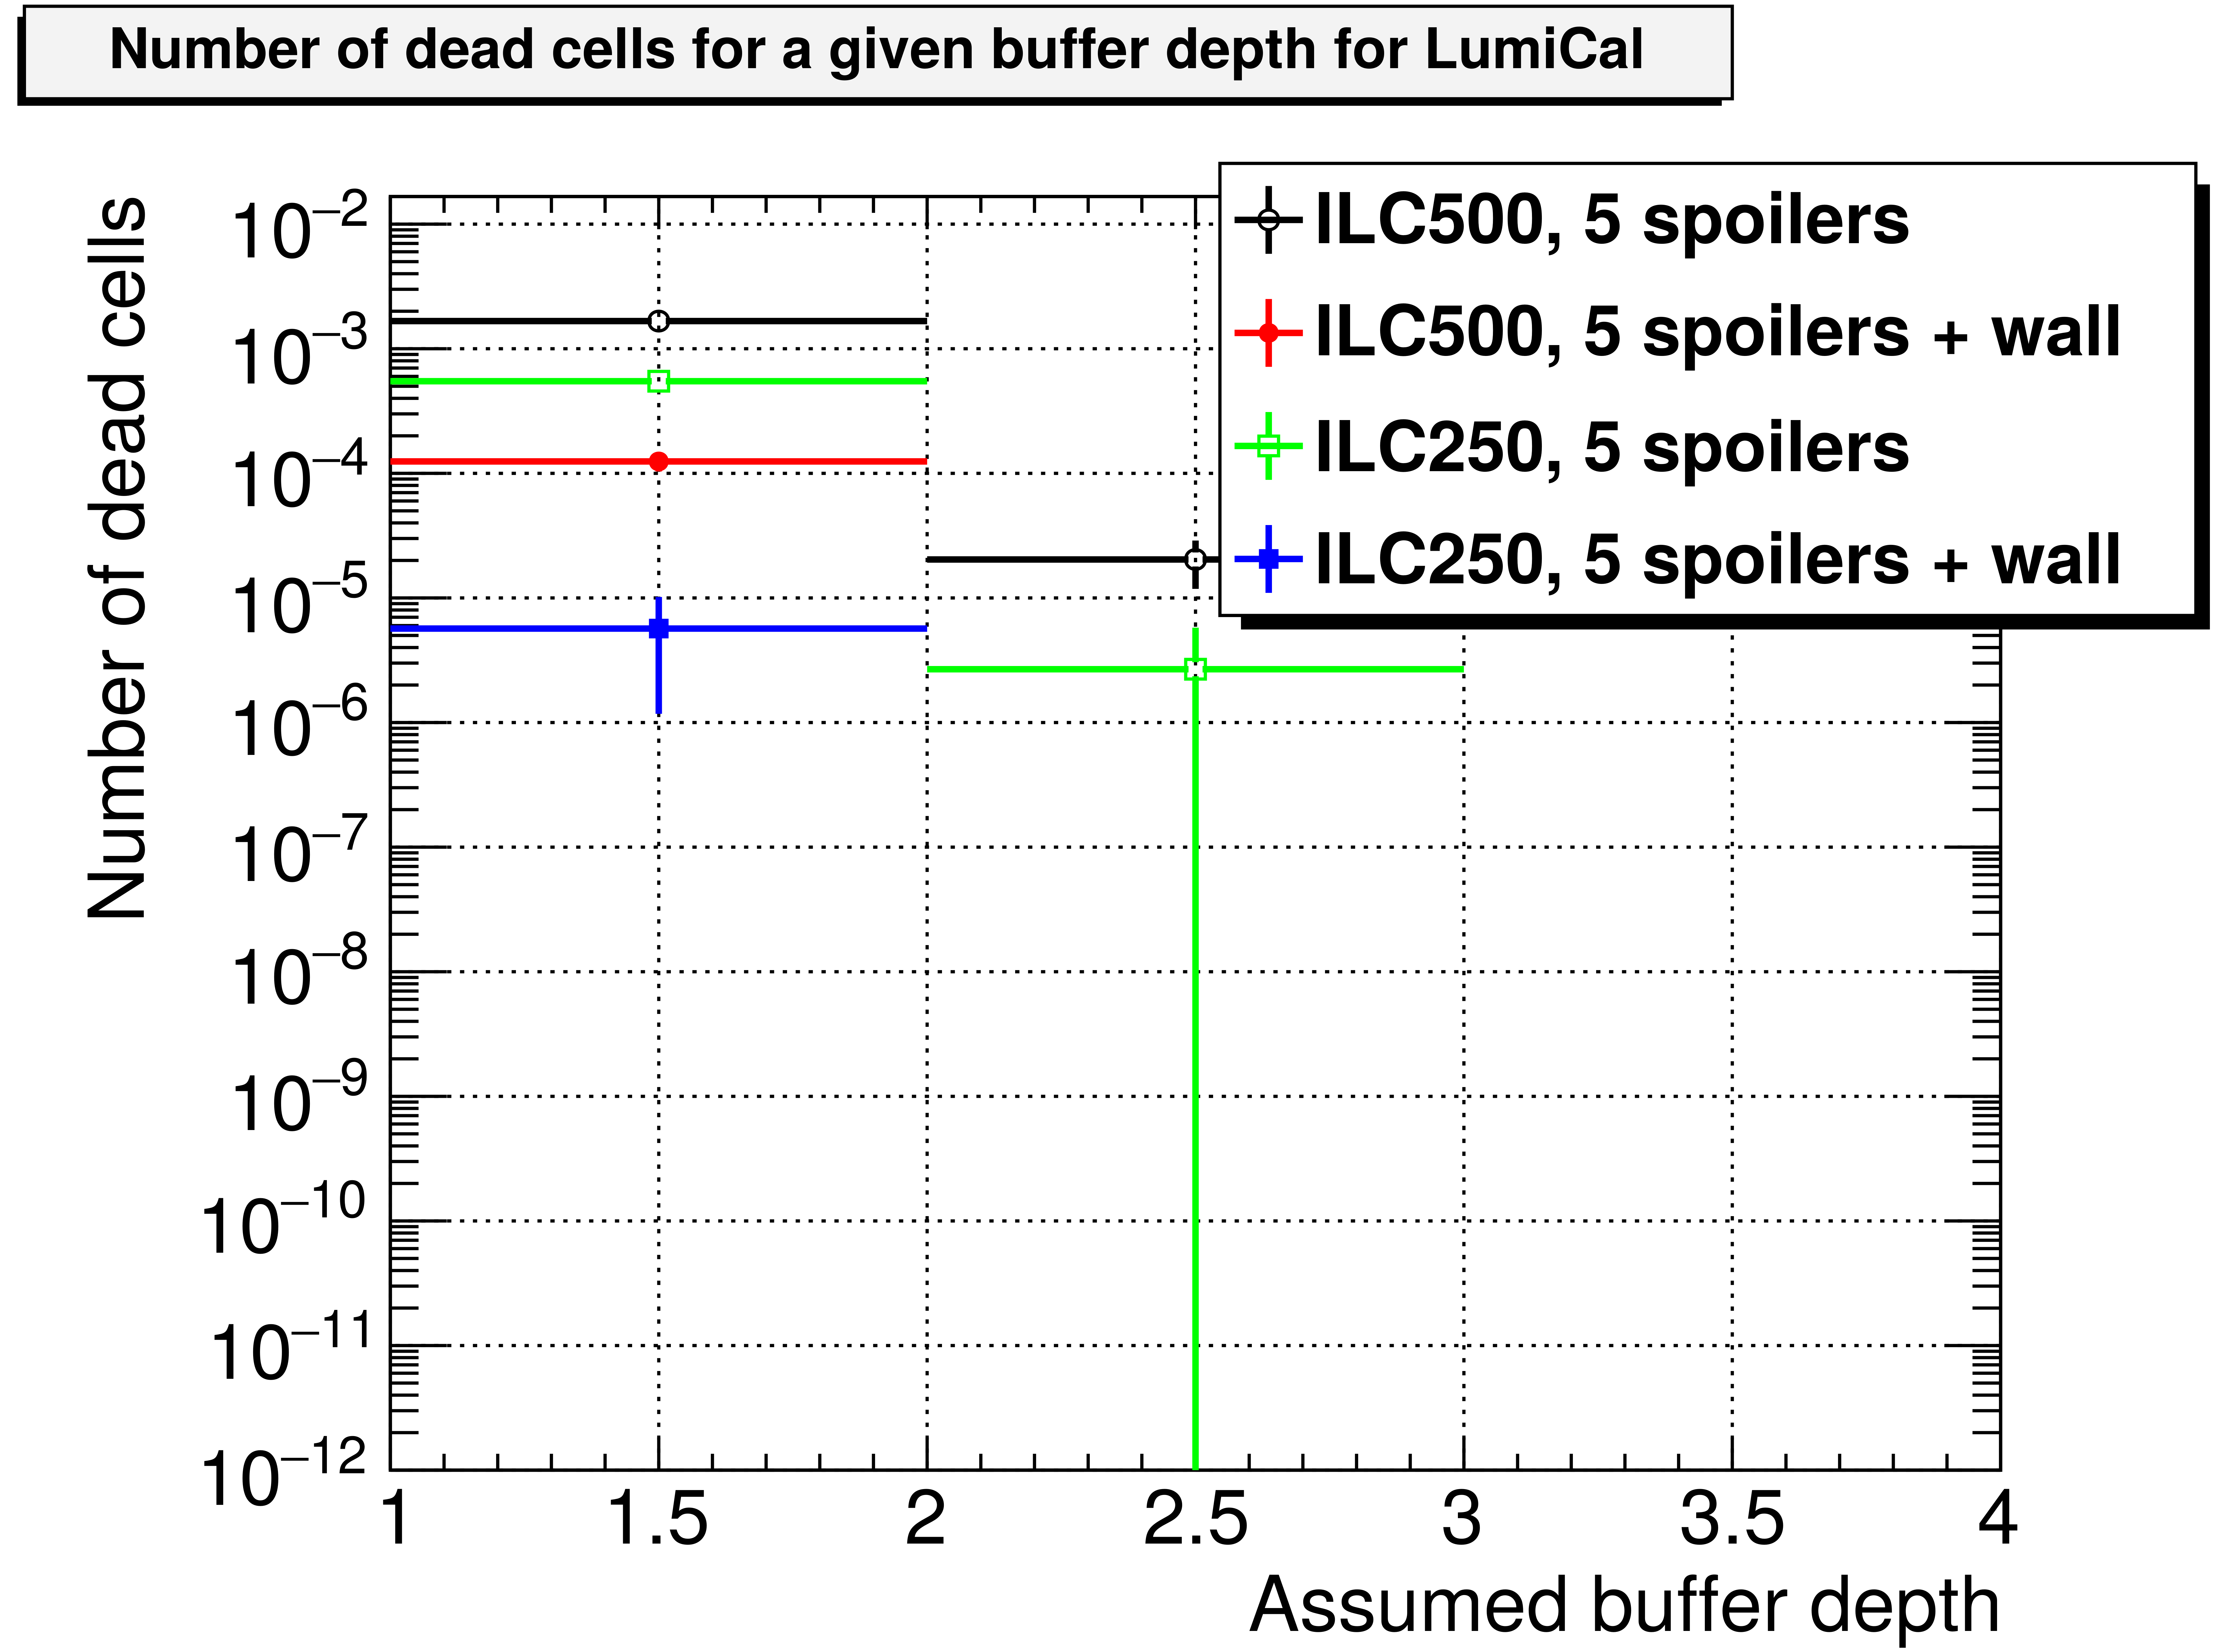
\includegraphics[width=\textwidth]{Figures/BDS_muons/Occupancy_Comparison_All_layers_deadcells_LumiCal.png}
   \caption{LumiCal}
   \end{subfigure}
   \caption[Occupancy from BDS muons of various SiD subdetectors]{The plots show the number of dead cells normalized by the total number of cells in the respective SiD subdetector.}
   \label{fig:BDS_Muons:occupancies}
 \end{figure}
 
\chapter{Background from the main beam dumps}
\label{Appendix:BeamDump}
\begin{figure}[!h]
 \centering
  \begin{subfigure}[b]{0.32\textwidth}
   \centering
    \includegraphics[width=\textwidth]{Figures/BeamDump/Design1_1.png}
   \caption{\designone, 1 minute}
   \end{subfigure}
   \hfill
    \begin{subfigure}[b]{0.32\textwidth}
   \centering
    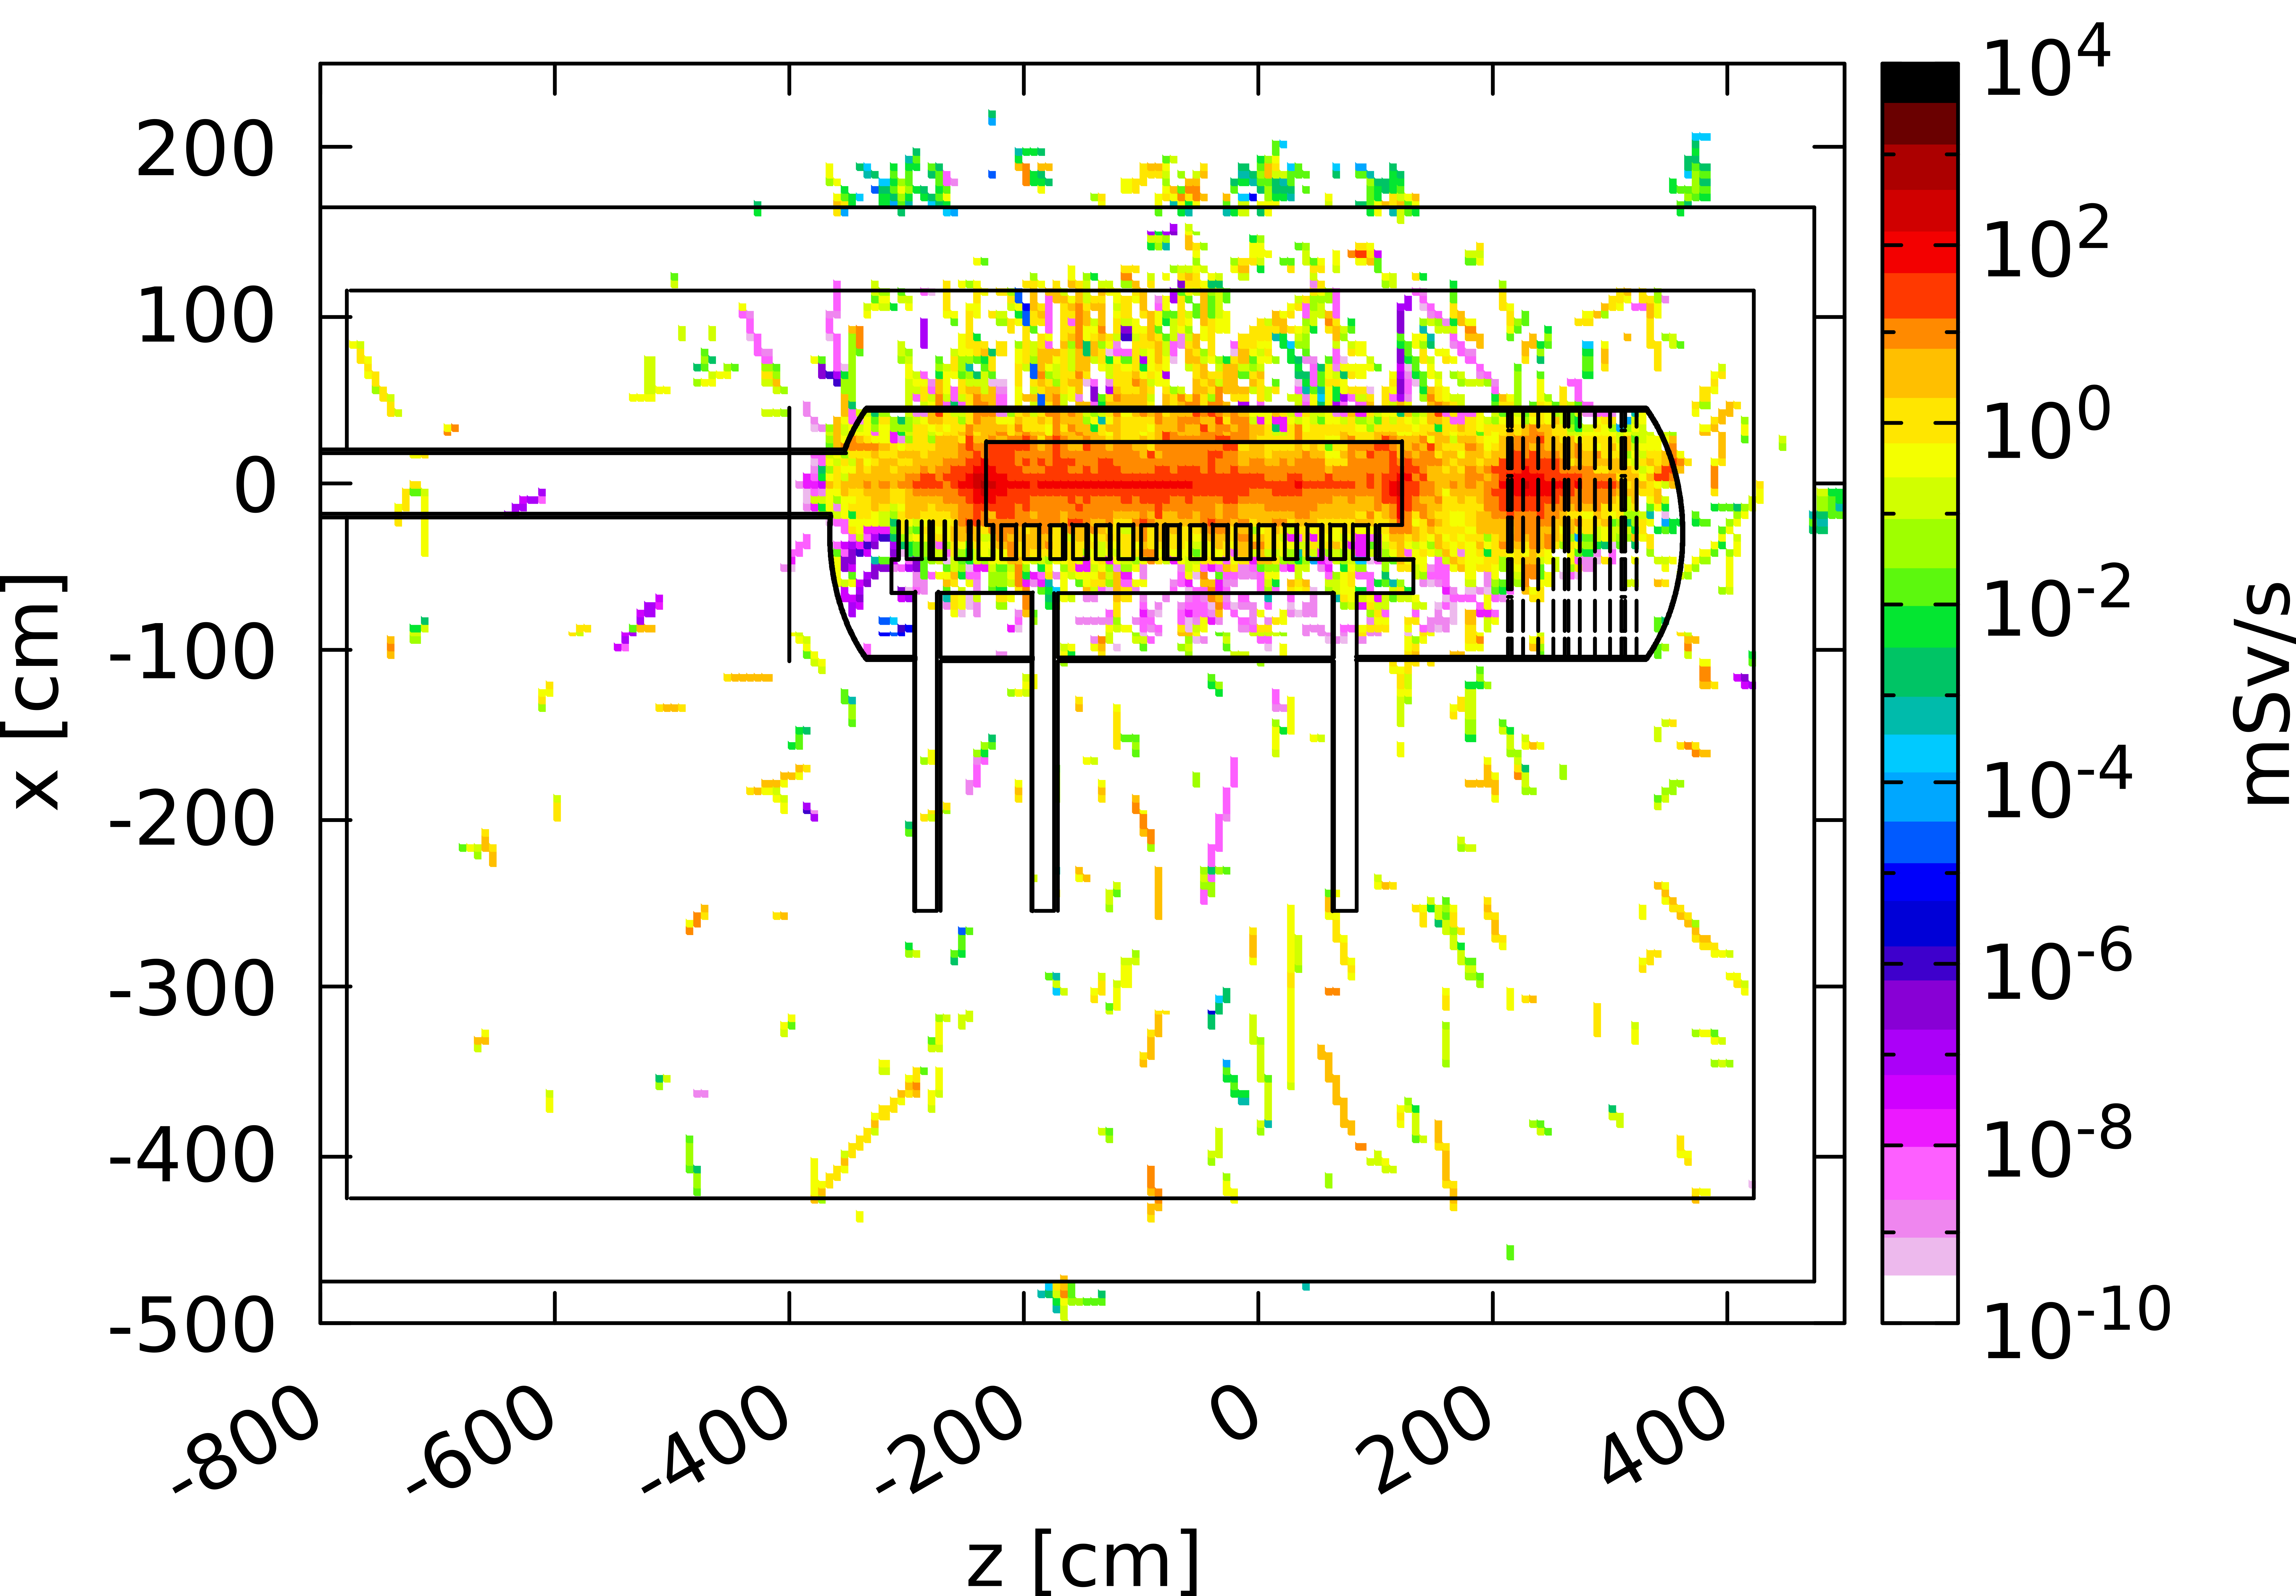
\includegraphics[width=\textwidth]{Figures/BeamDump/Design1_2.png}
   \caption{\designone, 1 hour}
   \end{subfigure}
      \hfill
     \begin{subfigure}[b]{0.32\textwidth}
   \centering
    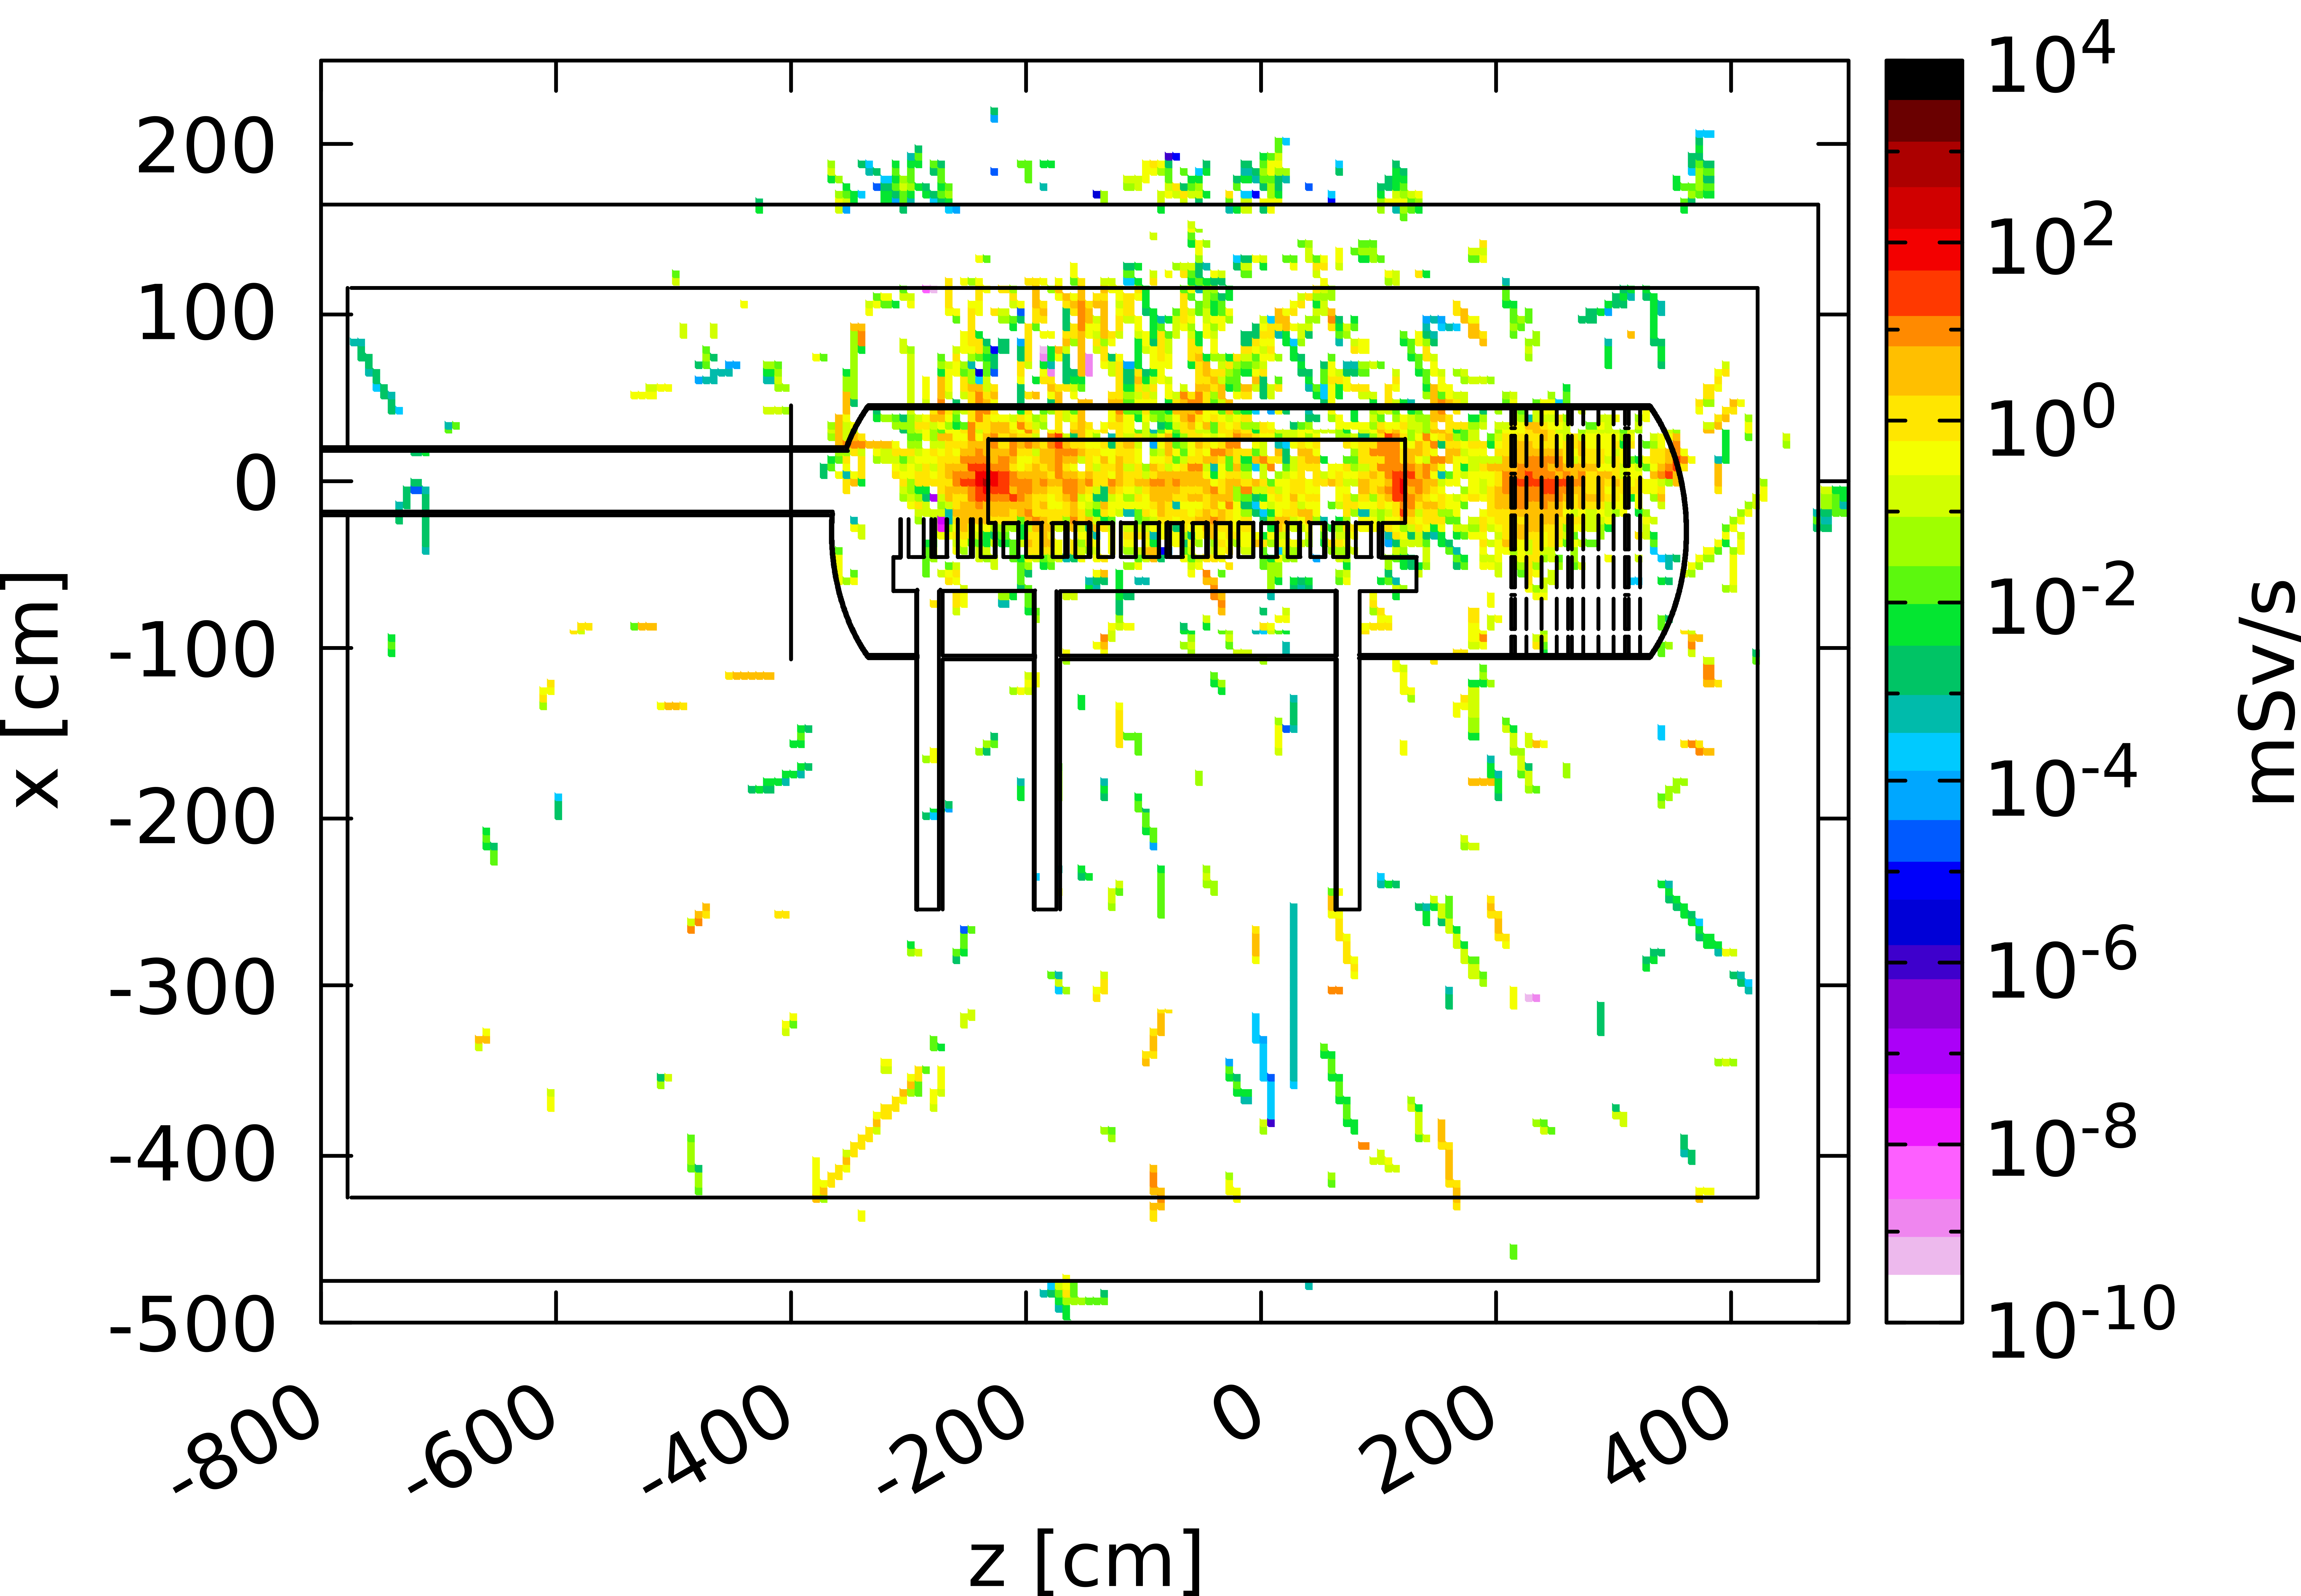
\includegraphics[width=\textwidth]{Figures/BeamDump/Design1_3.png}
   \caption{\designone, 1 day}
   \end{subfigure}\\ 
    \begin{subfigure}[b]{0.32\textwidth}
   \centering
    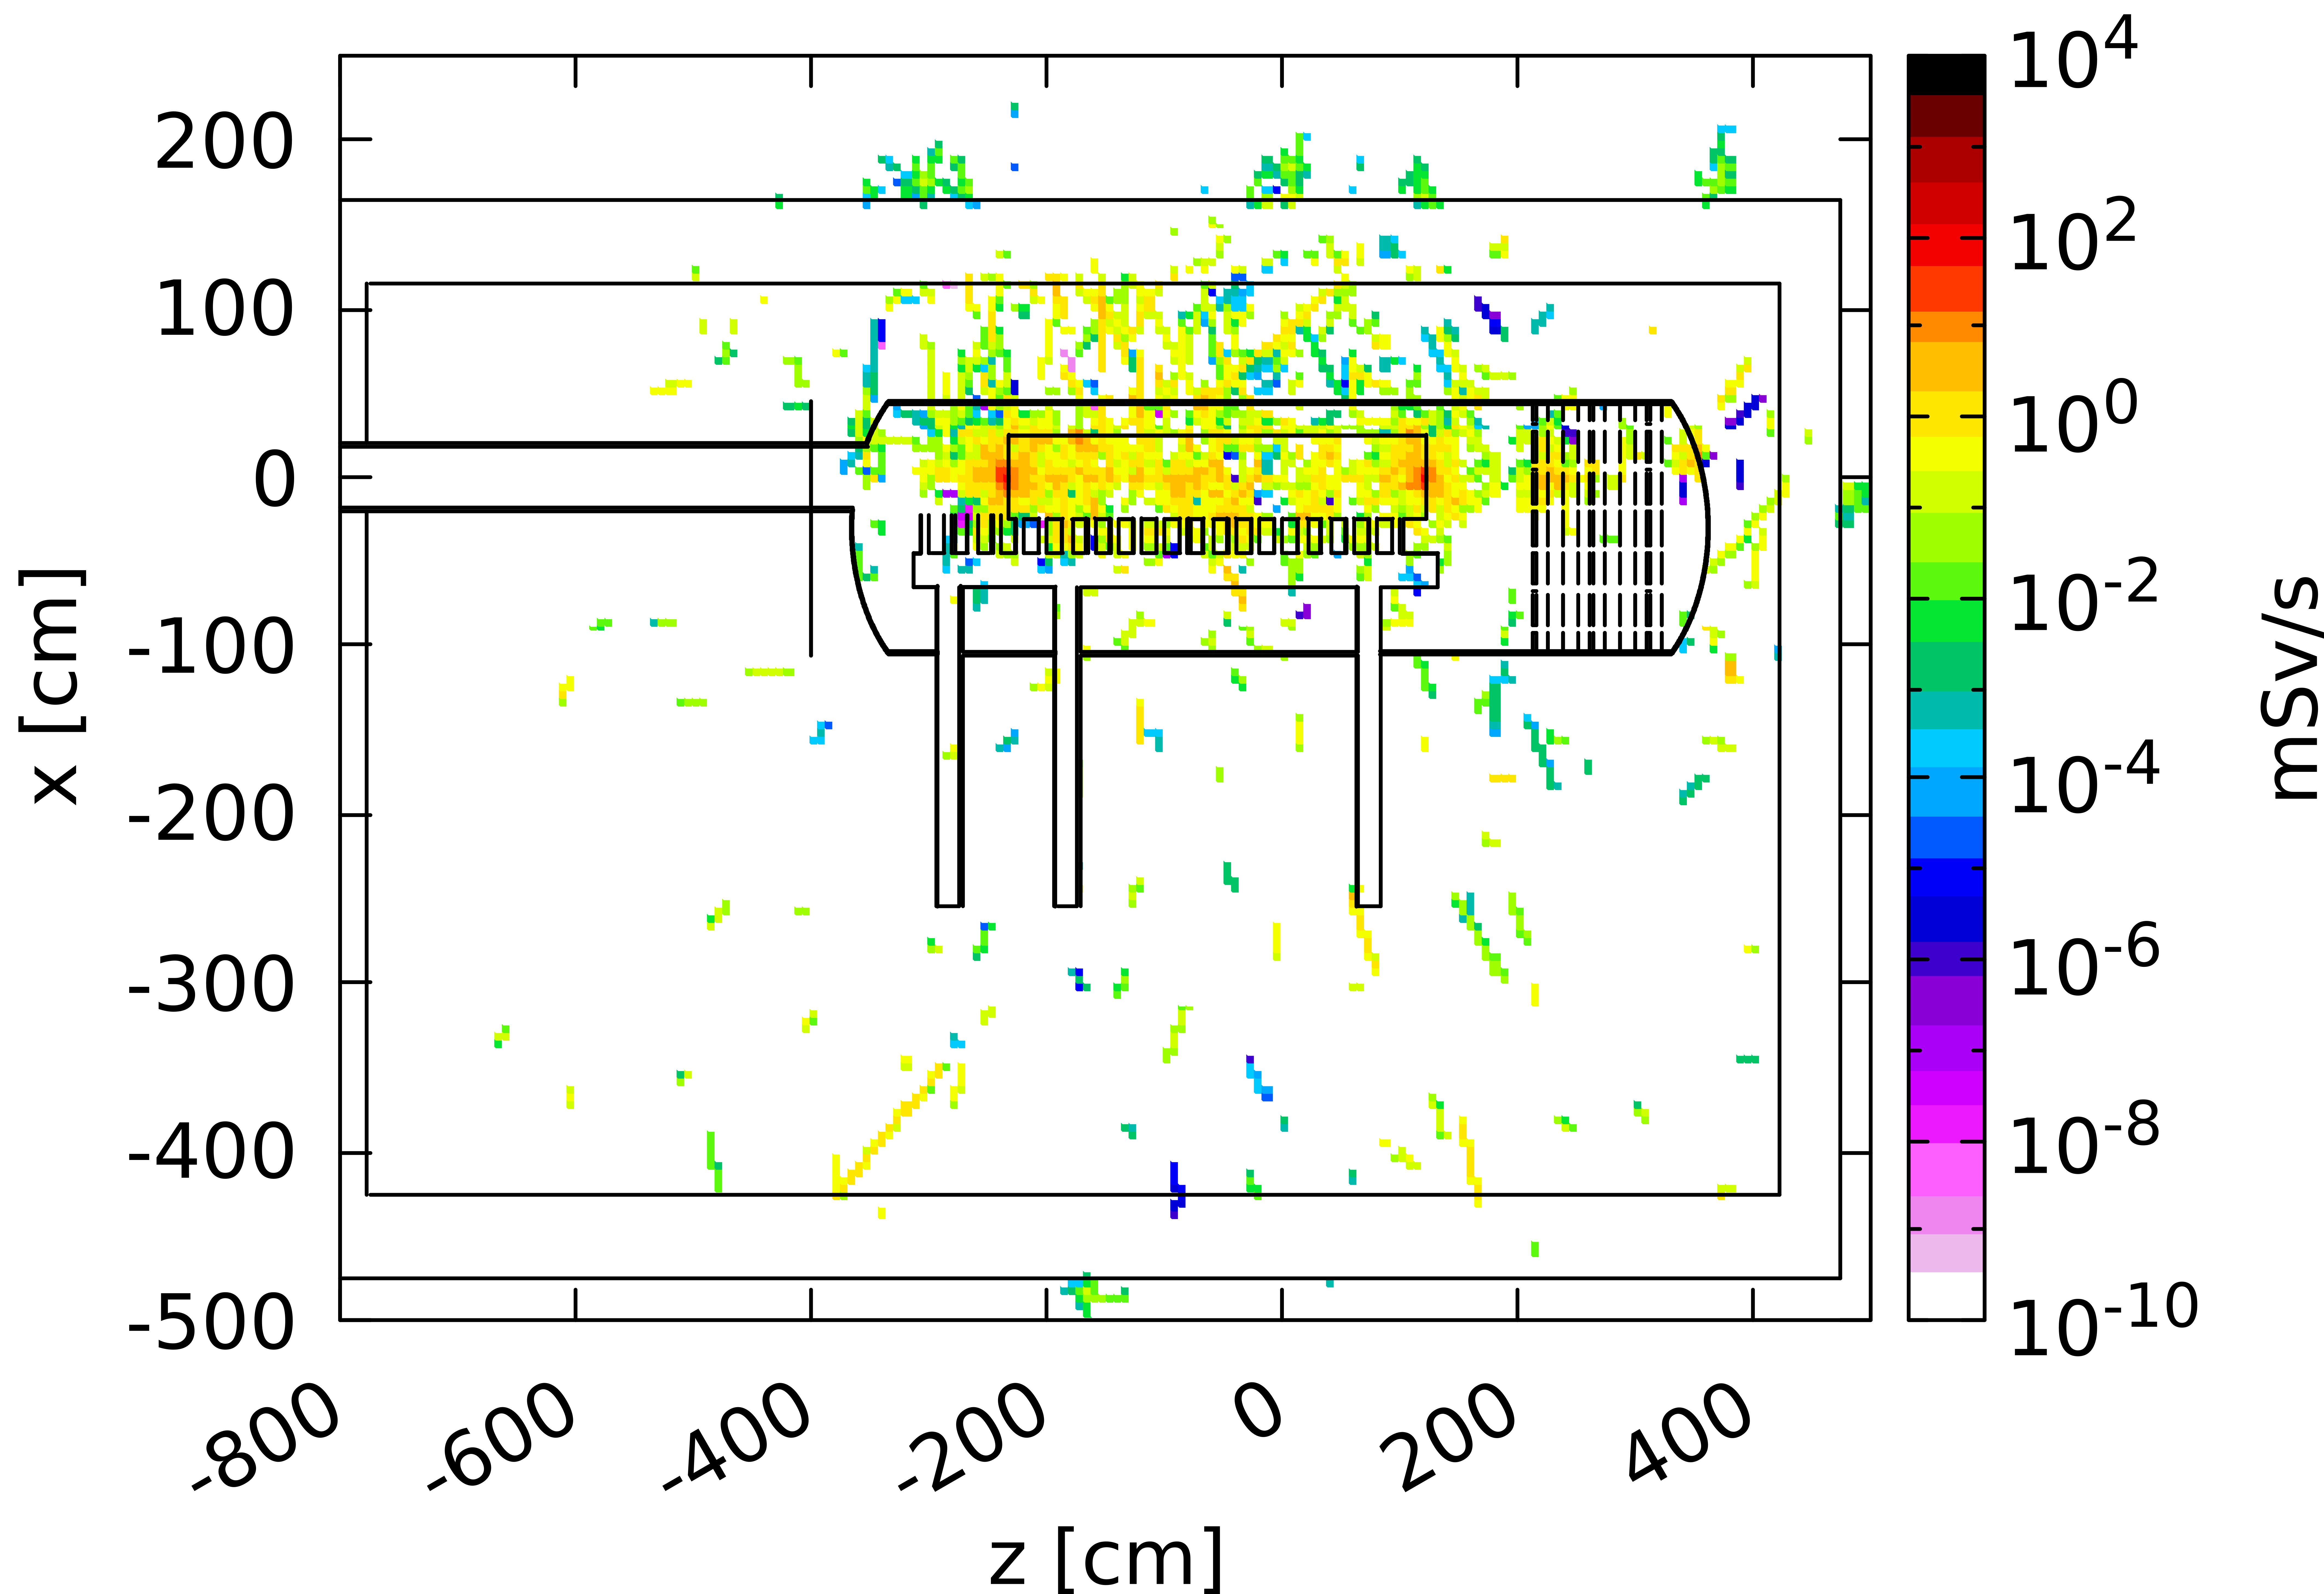
\includegraphics[width=\textwidth]{Figures/BeamDump/Design1_4.png}
   \caption{\designone, 1 month}
   \end{subfigure}
      \hfill
    \begin{subfigure}[b]{0.32\textwidth}
   \centering
    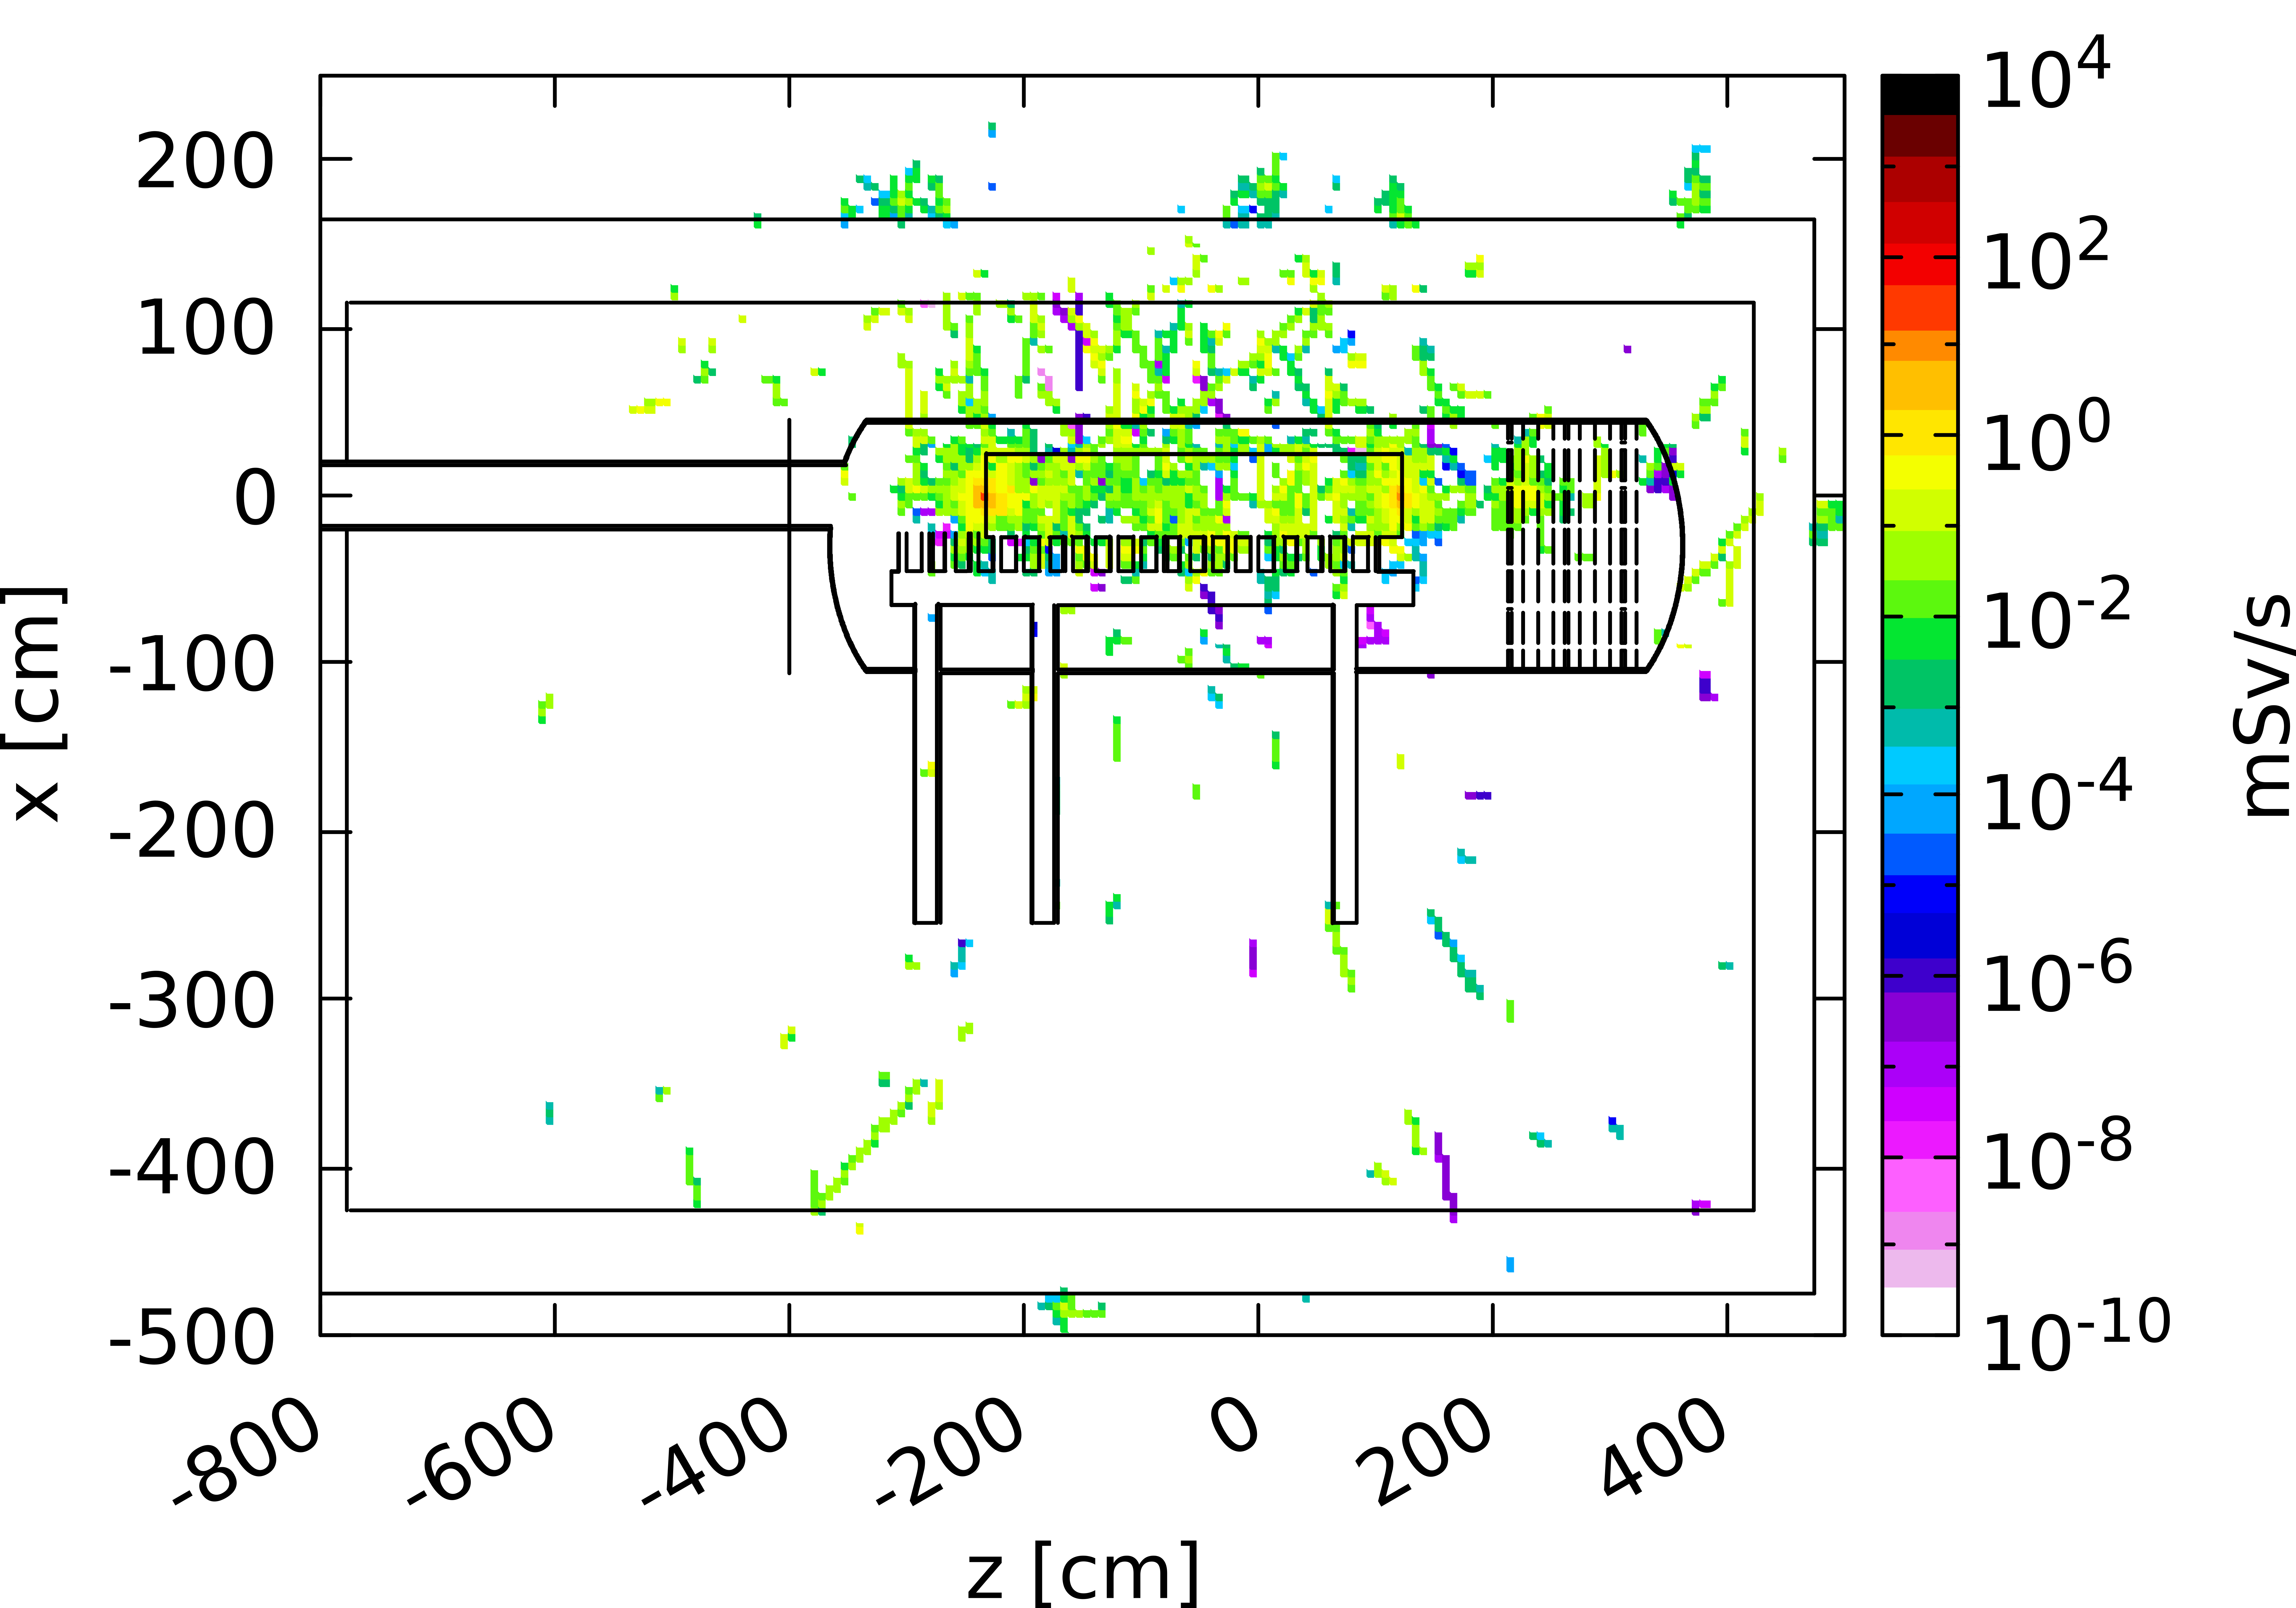
\includegraphics[width=\textwidth]{Figures/BeamDump/Design1_5.png}
   \caption{\designone, 1 year}
   \end{subfigure} 
   \hfill
   \begin{minipage}{0.32\textwidth}
   \hfill
    \end{minipage}
   \\
     \begin{subfigure}[b]{0.32\textwidth}
   \centering
    \includegraphics[width=\textwidth]{Figures/BeamDump/Design2_1.png}
   \caption{\designtwo, 1 minute}
   \end{subfigure}
   \hfill
    \begin{subfigure}[b]{0.32\textwidth}
   \centering
    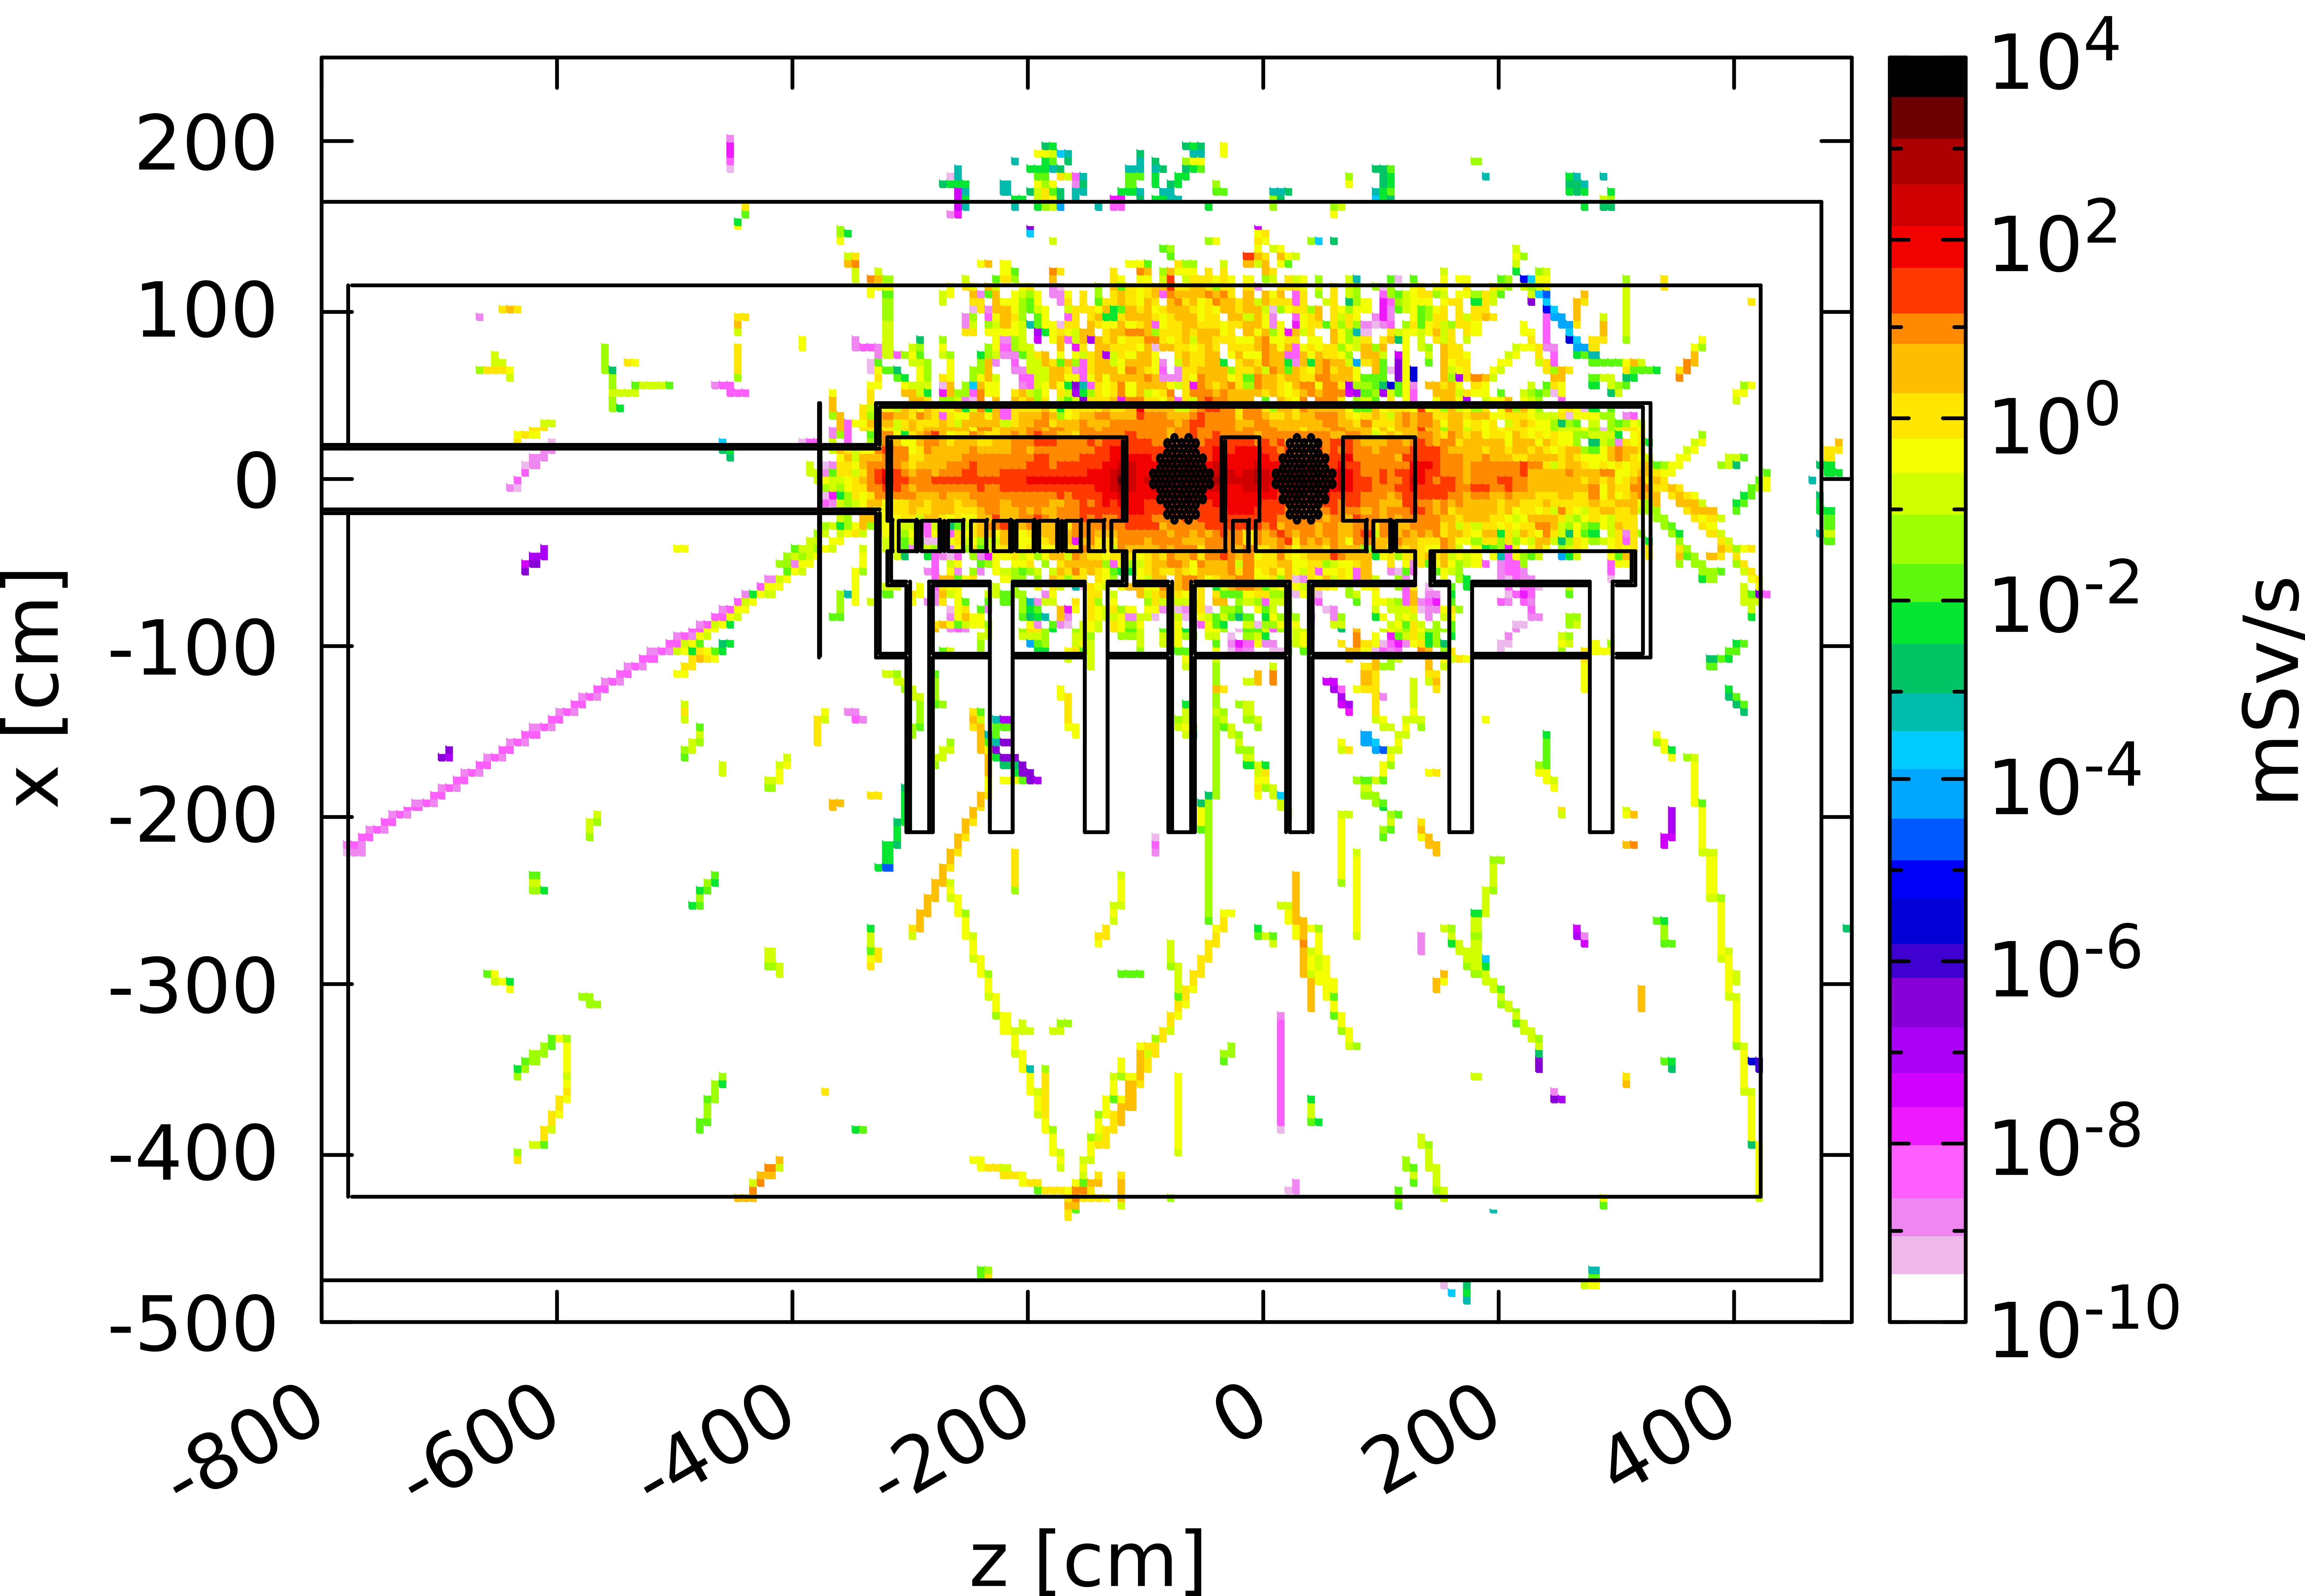
\includegraphics[width=\textwidth]{Figures/BeamDump/Design2_2.png}
   \caption{\designtwo, 1 hour}
   \end{subfigure}
      \hfill
     \begin{subfigure}[b]{0.32\textwidth}
   \centering
    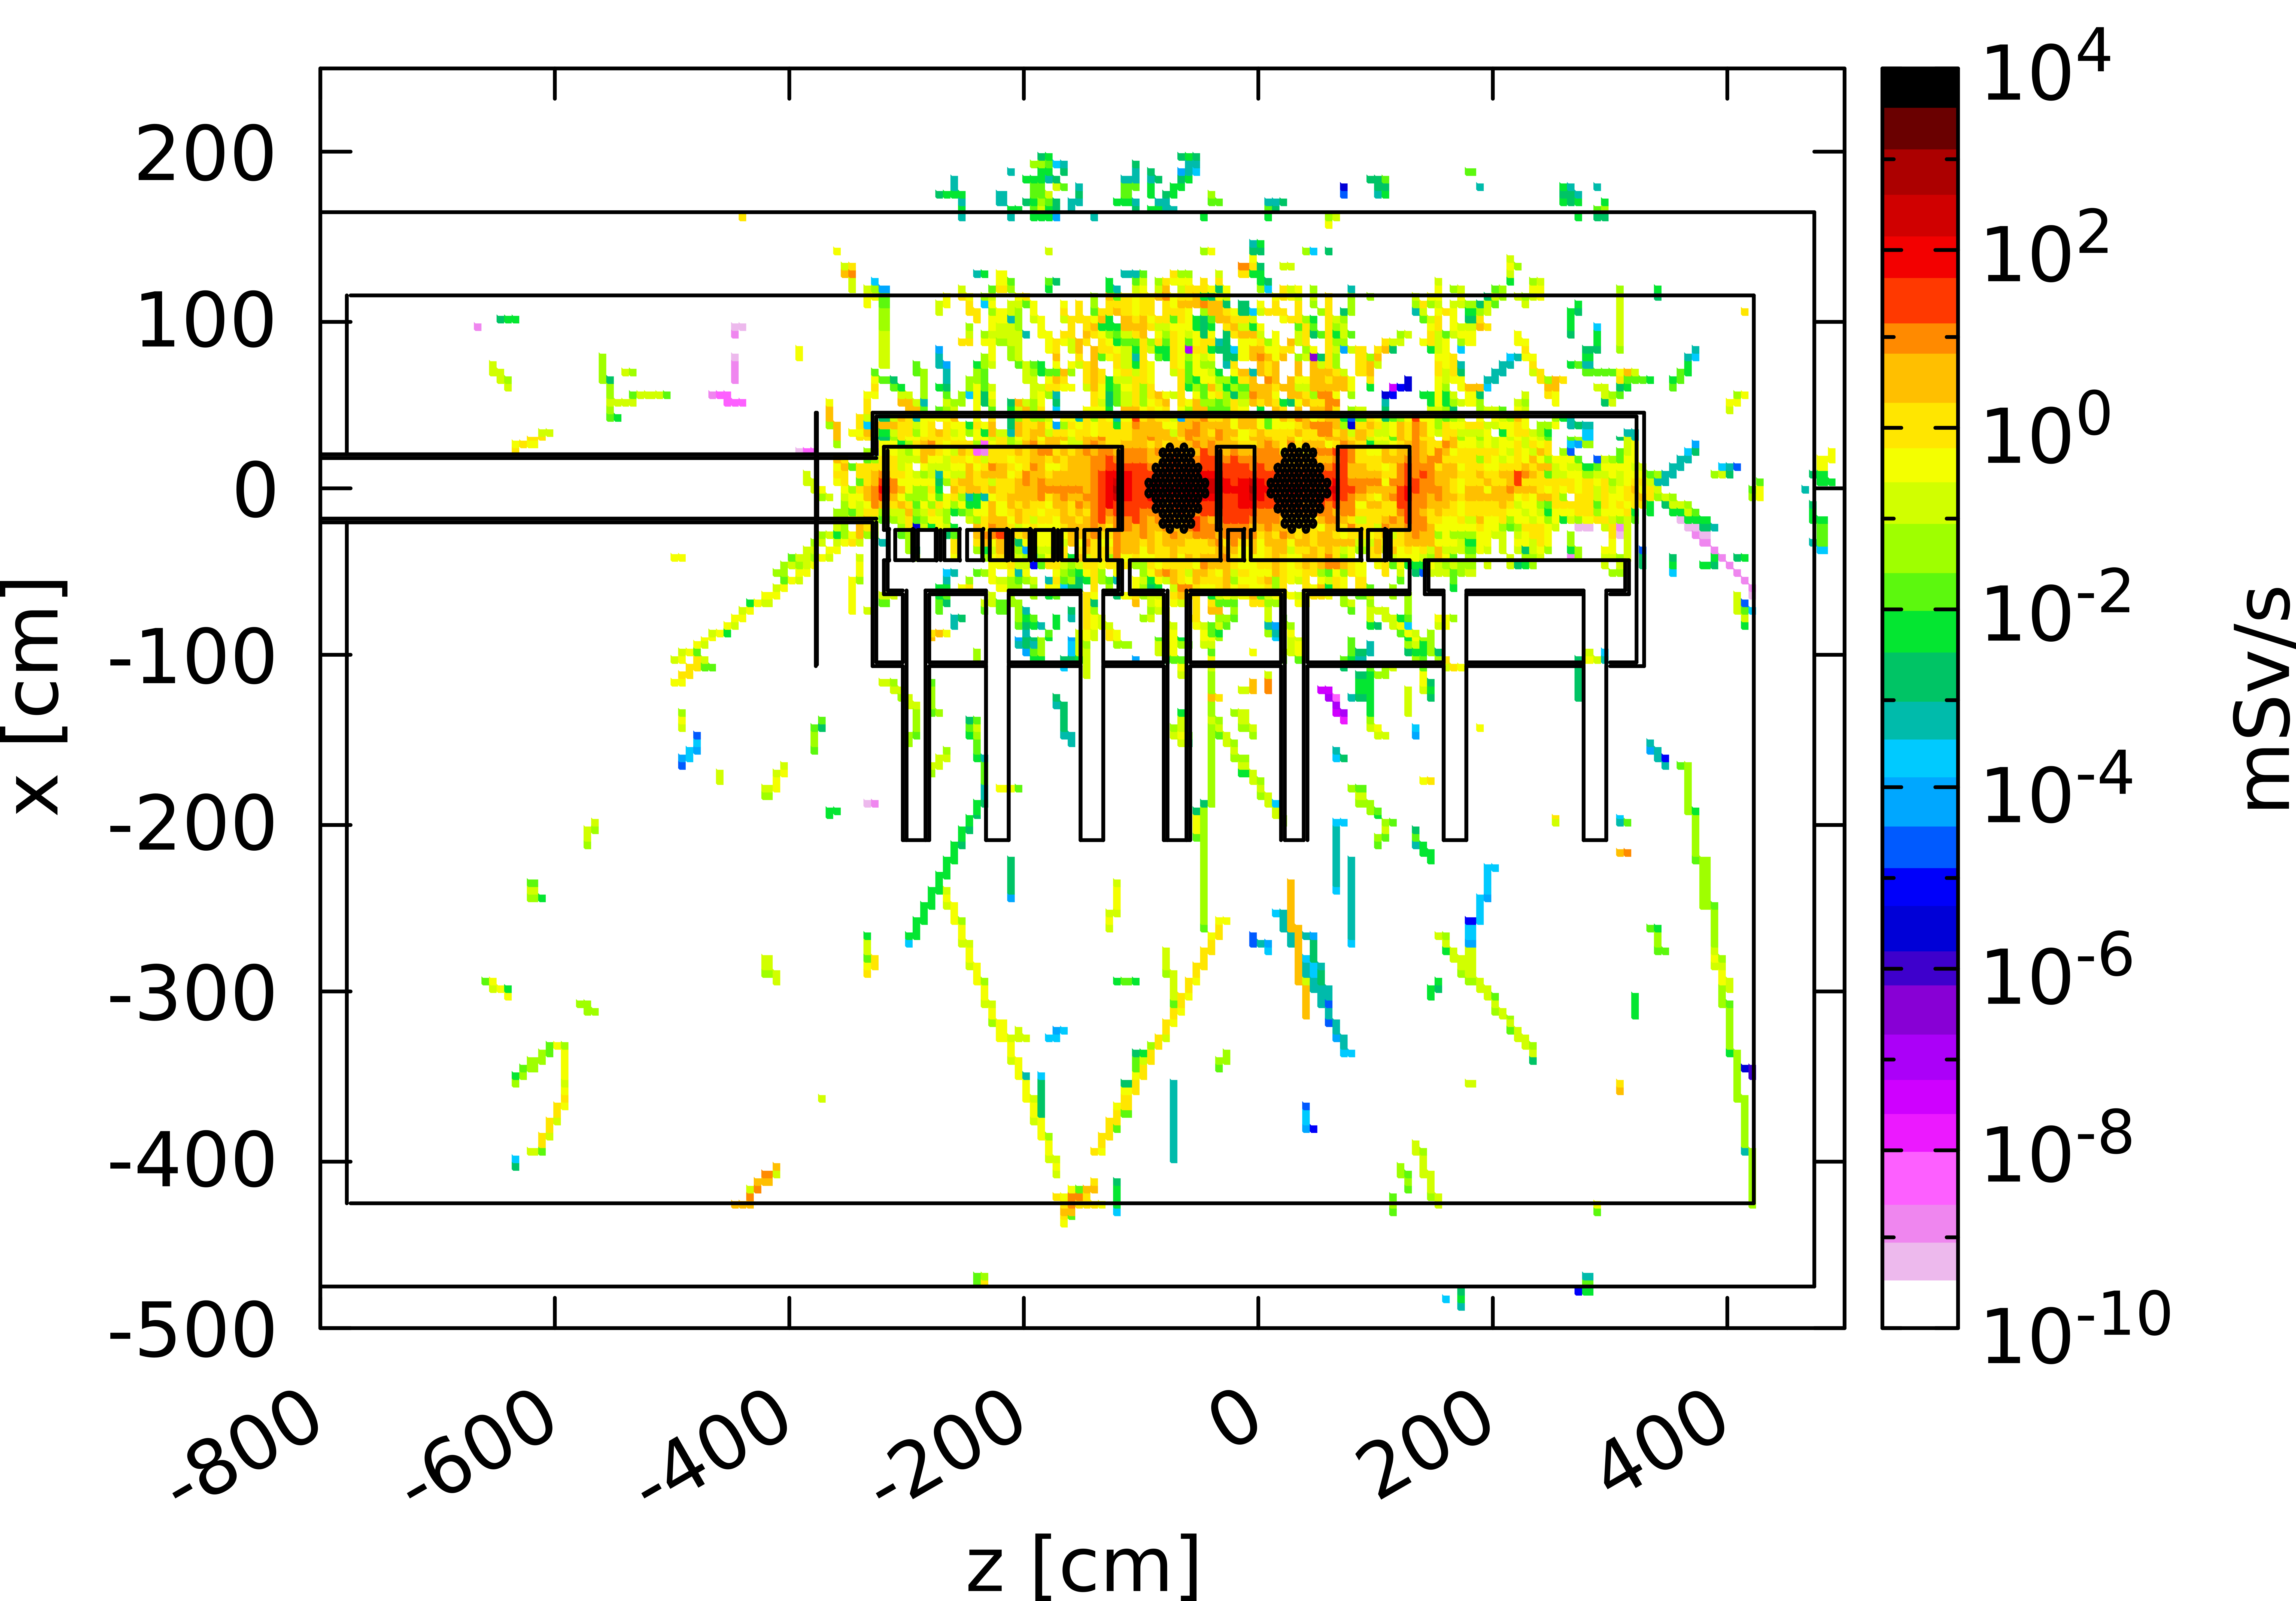
\includegraphics[width=\textwidth]{Figures/BeamDump/Design2_3.png}
   \caption{\designtwo, 1 day}
   \end{subfigure}\\
    \begin{subfigure}[b]{0.32\textwidth}
   \centering
    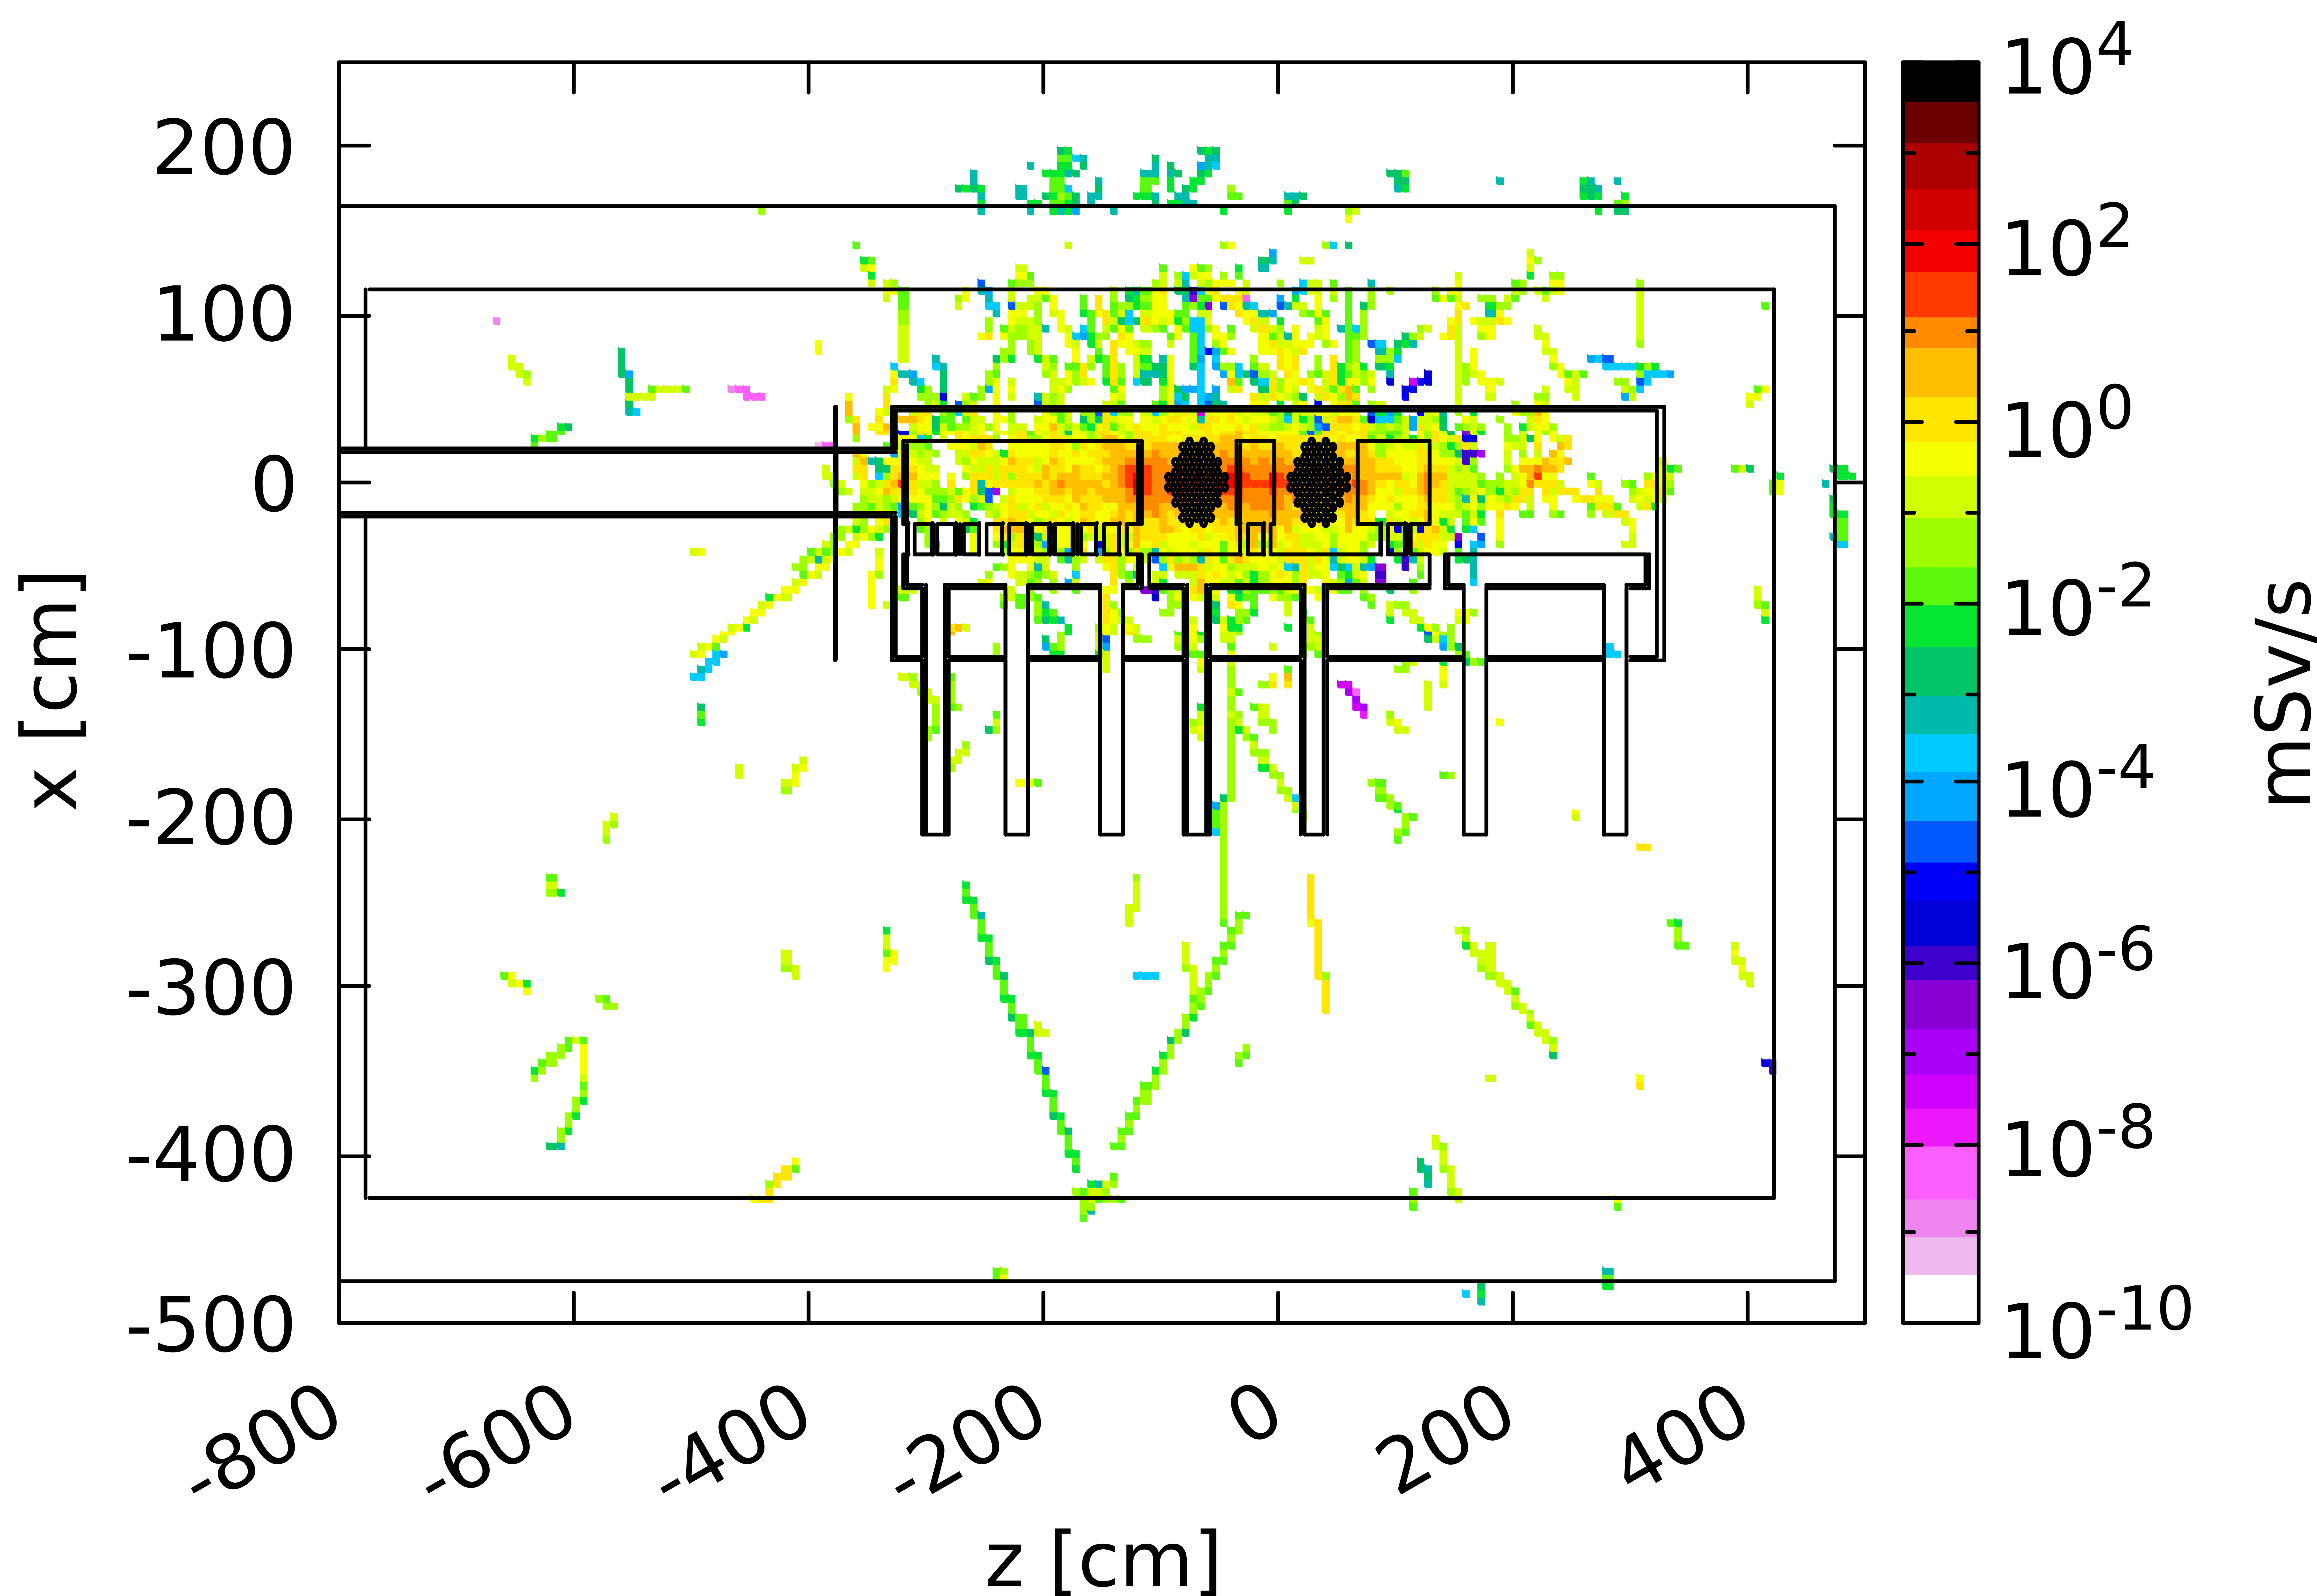
\includegraphics[width=\textwidth]{Figures/BeamDump/Design2_4.png}
   \caption{\designtwo, 1 month}
   \end{subfigure}
      \hfill
    \begin{subfigure}[b]{0.32\textwidth}
   \centering
    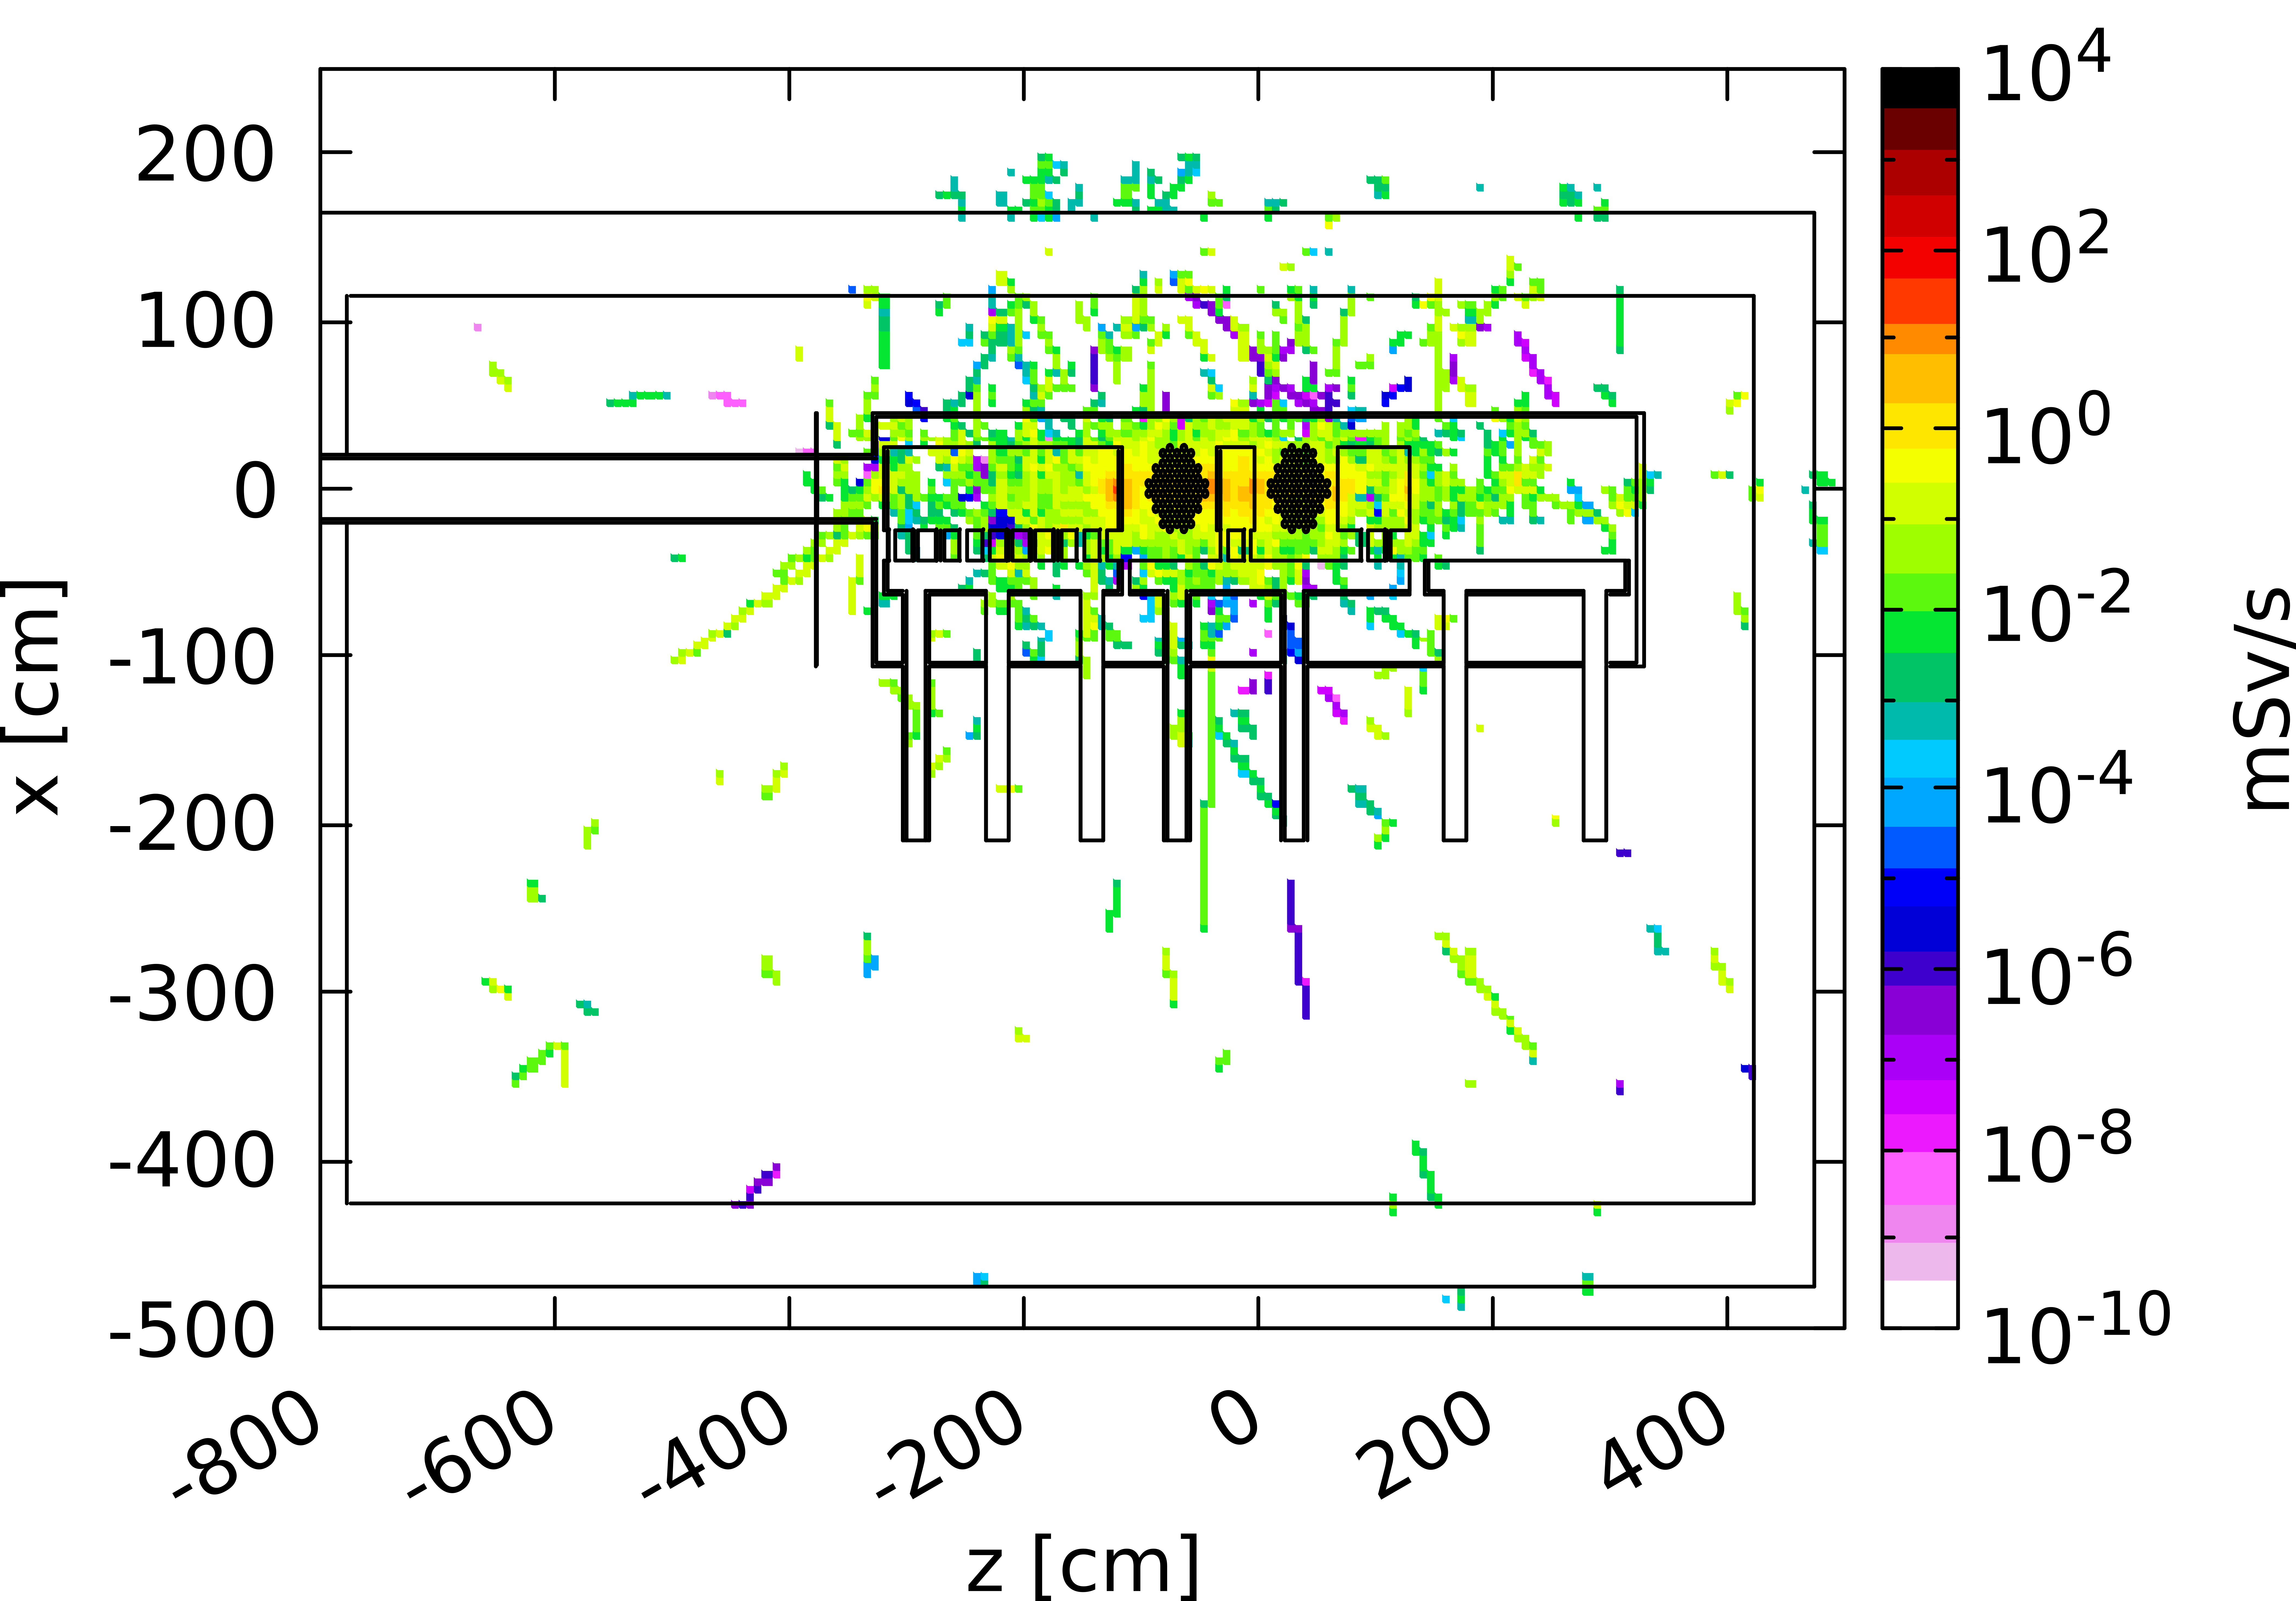
\includegraphics[width=\textwidth]{Figures/BeamDump/Design2_5.png}
   \caption{\designtwo, 1 year}
   \end{subfigure}
   \hfill
   \begin{minipage}{0.32\textwidth}
   \hfill
    \end{minipage}
   \caption[Dose rate in the ILC main beam dump after cooling times]{\fluka result of the dose rate in the ILC beam dump \designone (a) and \designtwo (b) and their surrounding after one month of beam operation and certain cooling times.
   The cooling times are given in the captions of the individual subfigures.
   The view is in the xz plane of the beam dump surrounding including the shielding walls.
   The color scale shows the dose rate in \si{\milli\sievert\per\second}.}
   \label{fig:BeamDumps:DoseRate}
\end{figure}